% Options for packages loaded elsewhere
\PassOptionsToPackage{unicode}{hyperref}
\PassOptionsToPackage{hyphens}{url}
\PassOptionsToPackage{dvipsnames,svgnames,x11names}{xcolor}
%
\documentclass[
  10pt,
]{article}
\usepackage{amsmath,amssymb}
\usepackage{lmodern}
\usepackage{iftex}
\ifPDFTeX
  \usepackage[T1]{fontenc}
  \usepackage[utf8]{inputenc}
  \usepackage{textcomp} % provide euro and other symbols
\else % if luatex or xetex
  \usepackage{unicode-math}
  \defaultfontfeatures{Scale=MatchLowercase}
  \defaultfontfeatures[\rmfamily]{Ligatures=TeX,Scale=1}
\fi
% Use upquote if available, for straight quotes in verbatim environments
\IfFileExists{upquote.sty}{\usepackage{upquote}}{}
\IfFileExists{microtype.sty}{% use microtype if available
  \usepackage[]{microtype}
  \UseMicrotypeSet[protrusion]{basicmath} % disable protrusion for tt fonts
}{}
\makeatletter
\@ifundefined{KOMAClassName}{% if non-KOMA class
  \IfFileExists{parskip.sty}{%
    \usepackage{parskip}
  }{% else
    \setlength{\parindent}{0pt}
    \setlength{\parskip}{6pt plus 2pt minus 1pt}}
}{% if KOMA class
  \KOMAoptions{parskip=half}}
\makeatother
\usepackage{xcolor}
\IfFileExists{xurl.sty}{\usepackage{xurl}}{} % add URL line breaks if available
\IfFileExists{bookmark.sty}{\usepackage{bookmark}}{\usepackage{hyperref}}
\hypersetup{
  pdftitle={A Functional Investigation of Species Richness Relationships in the North American Tree Flora},
  pdfauthor={Asger Svenning},
  colorlinks=true,
  linkcolor={Maroon},
  filecolor={Maroon},
  citecolor={Blue},
  urlcolor={blue},
  pdfcreator={LaTeX via pandoc}}
\urlstyle{same} % disable monospaced font for URLs
\usepackage[margin=1in]{geometry}
\usepackage{longtable,booktabs,array}
\usepackage{calc} % for calculating minipage widths
% Correct order of tables after \paragraph or \subparagraph
\usepackage{etoolbox}
\makeatletter
\patchcmd\longtable{\par}{\if@noskipsec\mbox{}\fi\par}{}{}
\makeatother
% Allow footnotes in longtable head/foot
\IfFileExists{footnotehyper.sty}{\usepackage{footnotehyper}}{\usepackage{footnote}}
\makesavenoteenv{longtable}
\usepackage{graphicx}
\makeatletter
\def\maxwidth{\ifdim\Gin@nat@width>\linewidth\linewidth\else\Gin@nat@width\fi}
\def\maxheight{\ifdim\Gin@nat@height>\textheight\textheight\else\Gin@nat@height\fi}
\makeatother
% Scale images if necessary, so that they will not overflow the page
% margins by default, and it is still possible to overwrite the defaults
% using explicit options in \includegraphics[width, height, ...]{}
\setkeys{Gin}{width=\maxwidth,height=\maxheight,keepaspectratio}
% Set default figure placement to htbp
\makeatletter
\def\fps@figure{htbp}
\makeatother
\setlength{\emergencystretch}{3em} % prevent overfull lines
\providecommand{\tightlist}{%
  \setlength{\itemsep}{0pt}\setlength{\parskip}{0pt}}
\setcounter{secnumdepth}{5}
\newlength{\cslhangindent}
\setlength{\cslhangindent}{1.5em}
\newlength{\csllabelwidth}
\setlength{\csllabelwidth}{3em}
\newlength{\cslentryspacingunit} % times entry-spacing
\setlength{\cslentryspacingunit}{\parskip}
\newenvironment{CSLReferences}[2] % #1 hanging-ident, #2 entry spacing
 {% don't indent paragraphs
  \setlength{\parindent}{0pt}
  % turn on hanging indent if param 1 is 1
  \ifodd #1
  \let\oldpar\par
  \def\par{\hangindent=\cslhangindent\oldpar}
  \fi
  % set entry spacing
  \setlength{\parskip}{#2\cslentryspacingunit}
 }%
 {}
\usepackage{calc}
\newcommand{\CSLBlock}[1]{#1\hfill\break}
\newcommand{\CSLLeftMargin}[1]{\parbox[t]{\csllabelwidth}{#1}}
\newcommand{\CSLRightInline}[1]{\parbox[t]{\linewidth - \csllabelwidth}{#1}\break}
\newcommand{\CSLIndent}[1]{\hspace{\cslhangindent}#1}
\usepackage[utf8]{inputenc} 
\usepackage[T1]{fontenc}
\usepackage{float}
\usepackage{wrapfig}
\usepackage{lipsum}
\usepackage{caption}
\usepackage[export]{adjustbox}
\usepackage{titling}
\usepackage{fancyhdr}
\usepackage{amsmath}
\usepackage{mathtools}
\usepackage{relsize}
\usepackage{changepage}
\usepackage{placeins}
\usepackage{hyperref}
\usepackage{todonotes}
\usepackage{tcolorbox}
\usepackage{textcomp}
\usepackage{threeparttable}

\pretitle{\begin{center}\LARGE}
\posttitle{\end{center}\vspace{2cm}\begin{center}
\includegraphics[width=12cm]{Aarhus_University_seal.png}\\[\bigskipamount]\end{center}\vspace{2cm}}
\preauthor{\begin{center}\large}
\postauthor{\end{center}\vspace{-0.25in}}
\predate{\begin{center}}
\postdate{\end{center}\begin{center}\huge\textcolor{RoyalBlue}{Aarhus University}\end{center}\newpage}

\DeclareCaptionFormat{custom}{
  \begin{tcolorbox}[
  colback=black!10,
  colframe=black!75,
  title=#1#2,
  arc=0pt,
  outer arc=0pt,
  boxrule=1pt,
  left=1pt,
  right=1pt,
  top=1pt,
  bottom=1pt,
  toptitle=3pt,
  bottomtitle=3pt
  ]
    \small #3
  \end{tcolorbox}
}
\DeclareCaptionLabelFormat{custom}
{
      \textbf{#1 #2}
}

\captionsetup{
    format=custom,
    labelformat=custom,
    labelsep=none,
    belowskip=-20pt
}

\renewcommand{\headrulewidth}{0pt}
\renewcommand{\thefootnote}{[\alph{footnote}]}
\renewcommand{\thefigure}{\arabic{figure}}
\renewcommand{\thetable}{\arabic{table}}

\pagestyle{fancy}

\fancyhead[L]{Asger Svenning}
\fancyhead[R]{\textcolor{RoyalBlue}{Aarhus University}}

\newcommand{\bquote}{\begin{adjustwidth}{0.05\textwidth}{0.05\textwidth}\centering}
\newcommand{\equote}{\end{adjustwidth}}


\newcommand{\aref}[1]{\hyperref[#1]{appendix~\ref*{#1}}}



\thispagestyle{empty}
\usepackage{booktabs}
\usepackage{longtable}
\usepackage{array}
\usepackage{multirow}
\usepackage{wrapfig}
\usepackage{float}
\usepackage{colortbl}
\usepackage{pdflscape}
\usepackage{tabu}
\usepackage{threeparttable}
\usepackage{threeparttablex}
\usepackage[normalem]{ulem}
\usepackage{makecell}
\usepackage{xcolor}
\ifLuaTeX
  \usepackage{selnolig}  % disable illegal ligatures
\fi

\title{A Functional Investigation of Species Richness Relationships in the North American Tree Flora}
\author{Asger Svenning}
\date{2022-06-11}

\begin{document}
\maketitle

\renewcommand*\contentsname{Table of Contents}
{
\hypersetup{linkcolor=}
\setcounter{tocdepth}{2}
\tableofcontents
}
\newpage

\hypertarget{introduction}{%
\section{Introduction}\label{introduction}}

\hypertarget{functional-analysis-ecosystem-functioning}{%
\subsection{Functional analysis \& Ecosystem functioning}\label{functional-analysis-ecosystem-functioning}}

Global crises are threatening critical ecosystem functioning for peoples and species on a global scale\textsuperscript{\protect\hyperlink{ref-IPBES2019}{1}}. Understanding the link between community composition and ecosystem services requires mapping functional attribute-space to ecosystem properties and derived downstream services\textsuperscript{\protect\hyperlink{ref-Lavorel2002}{2}}. By measuring the composition-function-service link, functional community ecology and biogeography could guide conservation ecology, by determining the possible changes to ecosystem-provided services as a result of biodiversity decline. Specifically, analyses of the patterns in functional traits are increasingly being used to investigate the interactions between ecology and evolution\textsuperscript{\protect\hyperlink{ref-Storch2019}{3},\protect\hyperlink{ref-Rabosky2015}{4}}, community assemblage patterns\textsuperscript{\protect\hyperlink{ref-Ricklefs2012}{5}--\protect\hyperlink{ref-Ordonez2018}{8}}, and drivers of ecosystem functioning\textsuperscript{\protect\hyperlink{ref-McGill2006}{9},\protect\hyperlink{ref-Paine2015}{10}}. Furthermore, functional ecology has been used to explain how species are distributed in niche-space, the drivers of these patterns and their connections to ecosystem services, and resilience to global change\textsuperscript{\protect\hyperlink{ref-Storch2019}{3},\protect\hyperlink{ref-McGill2006}{9},\protect\hyperlink{ref-Villeger2008}{11}--\protect\hyperlink{ref-Violle2014}{13}}. Therefore, functional ecology and biogeography has the potential to shape conservation actions by informing policymakers and other stakeholders of the value and vulnerability of species and ecosystems.

Functional analysis have been be applied at different ecosystem scales; from the local-community to biogeographical scale. At community scale, functional analysis are primarily used in local assessments or experiments, focused on explaining species coexistence patterns\textsuperscript{\protect\hyperlink{ref-McGill2006}{9},\protect\hyperlink{ref-Weiher1998}{14}}, ecosystem services\textsuperscript{\protect\hyperlink{ref-Scherer2008}{15},\protect\hyperlink{ref-Zavaleta2010}{16}} and invasiveness\textsuperscript{\protect\hyperlink{ref-Hejda2013}{17}}. Importantly, due to the local perspective and scale community centered studies can relatively easily obtain and integrate (relative) abundances\textsuperscript{\protect\hyperlink{ref-Weiher1998}{14}--\protect\hyperlink{ref-Zavaleta2010}{16},\protect\hyperlink{ref-Catford2019}{18}}. Additionally, these local efforts are often coupled with both site- and individual-based measurements of functional traits\textsuperscript{\protect\hyperlink{ref-Weiher1998}{14}}, which has been argued as being an important feature in functional analysis\textsuperscript{\protect\hyperlink{ref-Yang2018}{19}}.

The biogeographical perspective focuses on understanding the ecosystem-level effects of compositional changes due to past\textsuperscript{\protect\hyperlink{ref-Svenning2015}{20}} and ongoing\textsuperscript{\protect\hyperlink{ref-Culshaw2021}{21}} environmental changes, predicting vegetation types\textsuperscript{\protect\hyperlink{ref-Swenson2010}{22}}, ecosystem services\textsuperscript{\protect\hyperlink{ref-Paine2015}{10},\protect\hyperlink{ref-Violle2014}{13},\protect\hyperlink{ref-Yang2018}{19}} and investigating the relationship between niche-space and biodiversity patterns\textsuperscript{\protect\hyperlink{ref-Storch2019}{3}--\protect\hyperlink{ref-Ricklefs2012}{5},\protect\hyperlink{ref-Swenson2016}{7},\protect\hyperlink{ref-Ordonez2018}{8}}. In these approaches range maps or regional floras are often used to define the presence of species\textsuperscript{\protect\hyperlink{ref-Ricklefs2012}{5},\protect\hyperlink{ref-Ordonez2018}{8}}, given the limited number of datasets that summarize relative abundances for complete assemblages in a standardized way (see\textsuperscript{\protect\hyperlink{ref-Swenson2010}{22},\protect\hyperlink{ref-Swenson2012}{23}} for exceptions). Furthermore, biogeographical literature has, for the most part, intentionally limited the used trait databases to ecological attributes that define different and important functional dimensions\textsuperscript{\protect\hyperlink{ref-Swenson2016}{7},\protect\hyperlink{ref-Ordonez2018}{8},\protect\hyperlink{ref-Paine2015}{10},\protect\hyperlink{ref-Swenson2010}{22}--\protect\hyperlink{ref-Blonder2018}{24}}.

A key feature determining the difference between the community and biogeographical perspective is the use of abundances vs presence-only or presence/absence to define the topological attributes (i.e., variability and evenness) of the functional space under evaluation. The literature acknowledges that presence data will introduce biases in describing the functional space topological attributes\textsuperscript{\protect\hyperlink{ref-Swenson2016}{7}}, but these biases are poorly understood. However, as the amount of available occurrence data increases thanks to standardized large scale inventory protocols (e.g.~Forest Inventory and Analysis\textsuperscript{\protect\hyperlink{ref-FIADB}{25}} and breeding bird surveys\textsuperscript{\protect\hyperlink{ref-sauer2008north}{26},\protect\hyperlink{ref-Gillings2019}{27}}) and broad coverage (functional) trait databases (e.g.~PLANTS\textsuperscript{\protect\hyperlink{ref-PLANTS}{28}}, TRY\textsuperscript{\protect\hyperlink{ref-Fraser2020}{29}} and EltonTraits\textsuperscript{\protect\hyperlink{ref-Wilman2014}{30}}), we can now assess these biases.

This work investigates how shifting the focus from presences to abundance in functional analyses at biogeographic scales affects topological attributes of the functional space of woody plants in Eastern North America. This work will also determine how the size of the species pool and the evenness in the composition of the evaluated assemblages determine the discrepancies between presences and abundance estimates. The null expectation of this work is that integrating abundances will not result in greater than random increases in the functional space topological attributes that quantify central tendency and/or clustering in functional space. The alternative hypothesis is then, that integrating abundances will result in a greater than random increase in the central tendency and clustering of species in functional space, suggesting that presence data overly emphasizes rare and functionally unique species. The analyses and results presented here are intended to highlight when and how significant the use of abundances is when describing the functional space.

\hypertarget{methods-and-materials}{%
\section{Methods and Materials}\label{methods-and-materials}}

\hypertarget{data-sources}{%
\subsection{Data sources}\label{data-sources}}

To obtain an estimate of the relative abundances (quantified by individual counts) of woody plant species in the study region, I utilize the Forest Inventory and Analysis\textsuperscript{\protect\hyperlink{ref-FIADB}{25}} dataset, which includes over 22 million individual trees covering 418 species and varieties of woody plants across the contiguous Unites States from the period 1968-2021. The geographical size of this dataset allows for large-scale analysis (approximately 7.8 million square kilometers), while the large number of study units and individuals permits medium scale assemblage aggregation to a \(50 \times 50\) km grid using the NAD27 US National Atlas Equal Area coordinate projection. In order to aggregate the individual counts from different study units from different time periods, I have chosen to quantify the abundances as the number of individuals per plot per year using a two-step procedure; (1) individuals for each species in each grid cell for each year are tallied, (2) then I calculate the weighted mean of the tallies, by the number of study units in each grid cell for each year.

The abundance data is paired with the PLANTS trait-database\textsuperscript{\protect\hyperlink{ref-PLANTS}{28}}, which includes over 80 traits, of which I have deemed a subset (n = 50) to be both non-redundant and functionally relevant (more details in \aref{appendixTrait}). The utilized subset of traits are composed of 10 continuous and 40 ordinal/binary traits. These high quality data sources allows for a detailed analysis across a broad ecological range.

However, in the pool of species which are present in the FIA\footnote{In the contiguous US, not in e.g. Alaska.} data set only 123 of 372 have complete trait coverage in the PLANTS database. The remaining 249 species are missing trait information for an average of \textasciitilde23 traits per species. The missing values are imputed following a simple scheme; specifically missing values are imputed as the mean genus values of all woody plants species in the PLANTS dataset. Following this operation the average number of missing traits, for species with missing traits, is lowered to approximately 1.67 traits per species. Traits which still have more than a few missing values\footnote{1 out of every 50 species missing. This is the only parameter that was chosen manually in the procedure, and the specific value was chosen to balance the number of species and traits removed.} are then removed, followed by finally removing remaining species with missing values. This approach was chosen based on an assumption of phylogenetic conservatism and its simplicity, combined with the relatively low amount of values that needed to be imputed, due to the high initial trait coverage. Following the procedure the utilized data consisted of a total of 49 effective traits for 244 species across 68 genera. See \aref{appendixTrait} for further details on the traits used.

\hypertarget{functional-indices}{%
\subsection{Functional indices}\label{functional-indices}}

I have chosen to focus on the functional indices described in Villéger et al.~2008\textsuperscript{\protect\hyperlink{ref-Villeger2008}{11}} and Laliberté \& Legendre 2010\textsuperscript{\protect\hyperlink{ref-Laliberte2010}{31}} (functional dispersion, divergence, evenness and richness). I have chosen to mirror some of their methodological choices (using Gower dissimilarity as well as principal coordinate analysis for dimensionality reduction). A noteable methodological difference is that I use of Gower dissimilarity as the distance/dissimilarity measure for all indices, not only those that require dimensionality reduction, never Euclidean distance. This resolves a minor issue, which Laliberté \& Legendre themselves note:

\bquote

\emph{``FDis also satisfies all criteria but the first one (i.e., to be constrained between 0 and 1 for convenience) of Masonet al.~(2003) if traits are standardized prior to its computation\ldots{}''}\textsuperscript{\protect\hyperlink{ref-Laliberte2010}{31}}

\equote

Since Gower dissimilarity is itself constrained between 0 and 1 (unlike most other distance/dissimilarity measures, which are mostly constrained between 0 and +\(\infty\)), all four functional indices which I use in this project, are also restricted between 0 and 1 (see \aref{appendixGower} for further explanation). I interpret the functional indices as follows:

\begin{itemize}
\item
  \textbf{Functional dispersion (FDis)}: This metric is the is the average dissimilarity (``distance'') to the ``average'' (community weighted mean) species (i.e.~centroid) in functional space. Thus a lower functional dispersion corresponds to a stronger central tendency. Functional dispersion can then be understood as the degree to which species/individuals occupy a common niche within a community\textsuperscript{\protect\hyperlink{ref-Laliberte2010}{31}}.
\item
  \textbf{Functional evenness (FEve)}: This metric is the abundance-weighted evenness of the branch length of the minimum spanning tree (MST) of species in functional space. A high functional evenness is then achieved when the functional space is partitioned evenly\footnote{Along the minimum spanning tree.}, that is when species/individuals are uniformly spread \emph{not} clustered in functional space\textsuperscript{\protect\hyperlink{ref-Villeger2008}{11}}.
\item
  \textbf{Functional divergence (FDiv)}: This metric is a measure of the right-skewness of the dissimilarity from the un-weighted convex hull centroid distribution, and is strongly related to Rao's Quadratic Entropy (\textbf{Q}), however unlike \textbf{Q} functional divergence is not associated with functional richness\textsuperscript{\protect\hyperlink{ref-Mouchet2010}{12}}. A community with a high functional divergence then contains relatively many species/individuals which exhibit ``extreme'' functional traits\textsuperscript{\protect\hyperlink{ref-Villeger2008}{11}}.
\item
  \textbf{Functional Richness (FRic)}: This metric is the convex hull hypervolume of the set of species in a community. Functional richness then measures the size of the utilized niche-space in a community\textsuperscript{\protect\hyperlink{ref-Villeger2008}{11}}.
\end{itemize}

\hypertarget{modelling}{%
\subsection{Statistical modelling}\label{modelling}}

\begin{figure}
  \vspace{-0.6cm}
  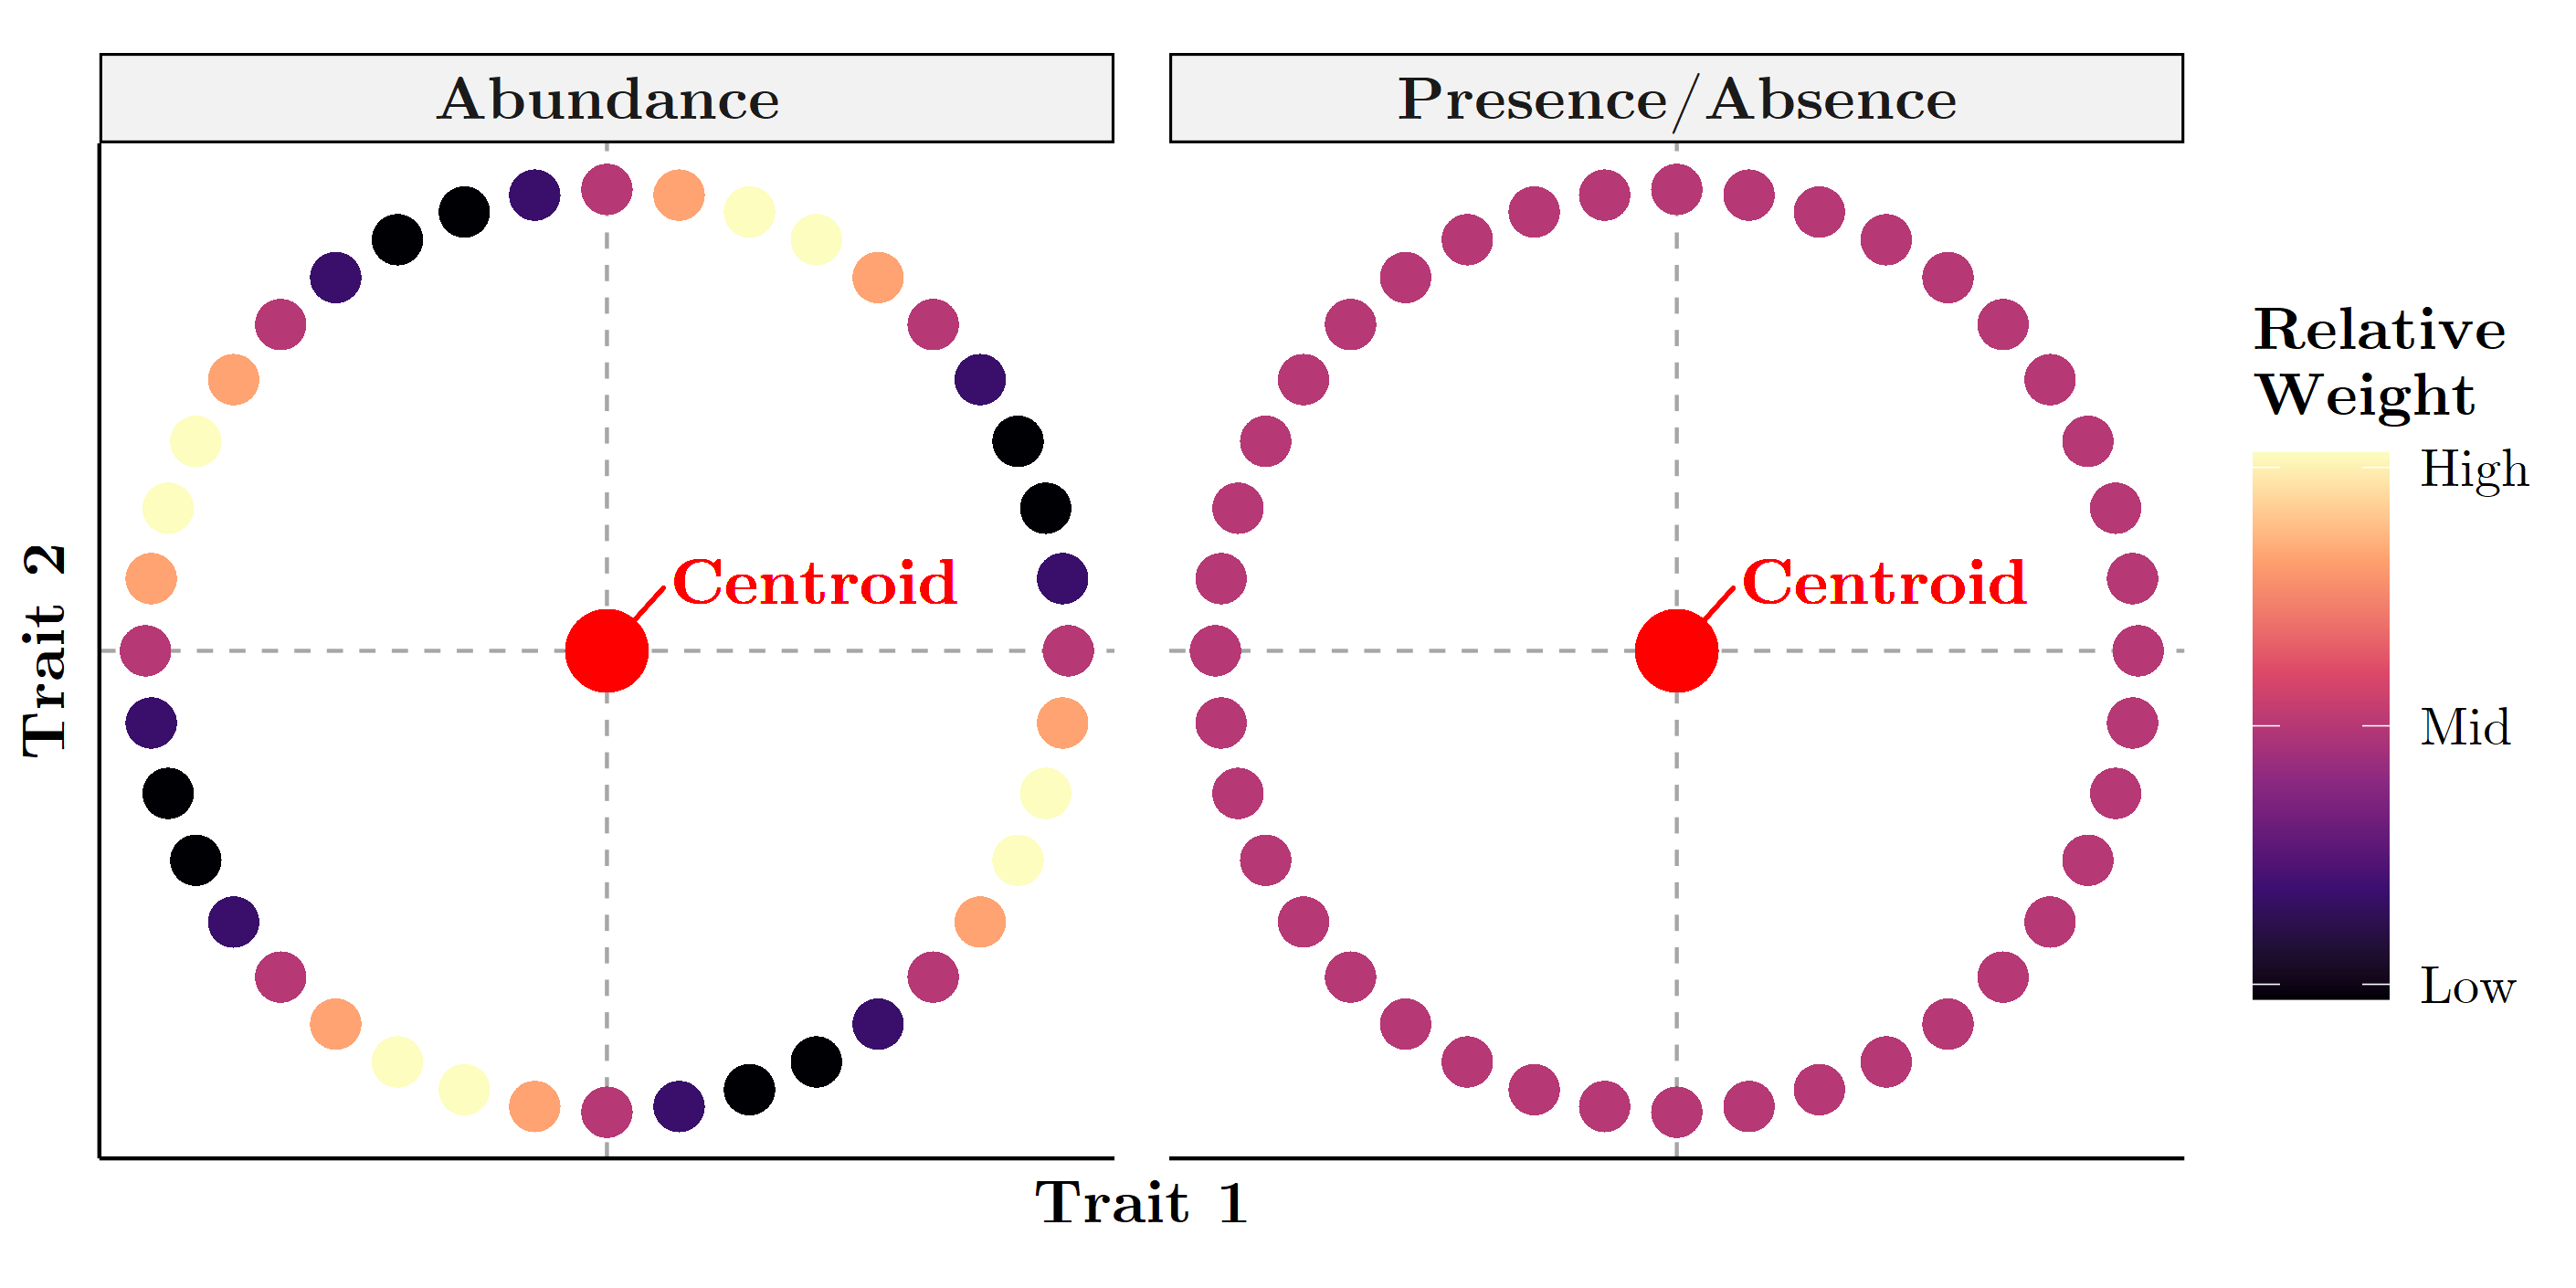
\includegraphics[width=\linewidth]{../Final Visualizations/exampleNoChangeFDis.png}
  \caption{Functional dispersion does not necessarily change based on weights. It is not obvious for which, if any, of the functional indices, a Shannon evenness of less than one, is a sufficient condition for a change in the value of the index. For this purpose I have constructed a set of species, which are distributed in a manner in which all distances to the centroid are equal, and a set of uneven weights, which do not result in a shift in the centroid location.}
  \label{fig:counterExample}
  \vspace{.35cm}
\end{figure}

To capture the environmental gradients in the analyses, I disaggregate the results across different ``ecosystems'' based on the EPA ecoregion framework\textsuperscript{\protect\hyperlink{ref-EPAecoregions}{32}}. I found that the EPA ecoregions delineate distinct woody plant assemblages or ecosystems at the scale of my analysis (\(50\times50\) km grid), based on a support vector machines (SVM) classification on the relative abundance vectors. Before classification the abundance vectors are ordinated using principal coordinate analysis\footnote{The dissimilarity metric is Bray-Curtis, i.e. manhattan distance divided by two.}, and the number of axes are determined based on a broken stick approach (n = 18). The repeated (n=5) k-fold (k=5) cross-validation accuracy is between {[}0.819, 0.976{]} with a mean of 0.935\footnote{This approach is chosen over the more classical linear discriminant analysis, since this has a much lower minimum and mean CV accuracy of [0.161, 0.927] \& 0.64.}. The confusion matrix for the SVM model can be found in \aref{appendixConfusion}, also visually confirms the validity of the result.

I calculate the functional indices (FDis, FDiv, FEve \& FRic) for all communities (grid cells) twice, once with the relative abundances from FIA and once where all abundances that are not zero are standardized to one, i.e.~presence data. Conceptually the standardization of abundances is then treated as a ``treatment'' and each grid cell as a replicate. I define bias in the context of this procedure as the difference between the functional index value given the true abundances and the standardized ``presence'' abundances for a grid cell; \(\mathrm{Bias}: \mathrm{Index_{Abundance}} - \mathrm{Index_{Presence}}\). To determine the drivers of bias in the functional indices I have chosen to use generalized additive mixed models (GAMM), due to their great flexibility in mixing parametric, semi-parametric (here thin plate regression splines\textsuperscript{\protect\hyperlink{ref-R-mgcv-5}{33}}) and random effects\textsuperscript{\protect\hyperlink{ref-R-gamm4}{34}}. Semi-parametric terms and random effects are used only to account for spatial autocorrelation, imbalanced sampling and pseudo-replication. Species richness is first log-transformed and then both Shannon Evenness and species richness are scaled and modelled as fixed linear effects. These models were formalized as: \(y = X\boldsymbol{\beta} + \boldsymbol{\zeta} + \varepsilon\), where \(X\boldsymbol{\beta}\) are the fixed parametric effects and \(\boldsymbol{\zeta}\) are the semi-parametric and random effects. \(\boldsymbol{\zeta}\) is composed of two terms; \(\mathbf{\zeta} = \hat{f}(x,y,\log(\mathrm{N_{samples}}))+Z\mathbf{u}\), where \(\hat f\) is a smoothing term (thin plate splines) of the geographic coordinates (\(x,y\)) and the logarithm of the number of FIA plots in a grid cell (\(\log(\mathrm{N_{Samples}})\)), while \(Z\mathbf{u}\) is a random effect term of grid cell ID nested in Ecoregion. The smoothing term is included to account for spatial as well as sampling patterns in both the value and bias of the index. The initial model formulation was then:
\[\mathrm{Index} \sim \mathrm{Type} + s(x,y,\mathrm{N_{samples}}) + (1\,|\,\mathrm{Ecoregion/Type})\]

\begin{wrapfigure}[]{l}{0.5\textwidth}
  \vspace{-0.5cm}
  \centering
  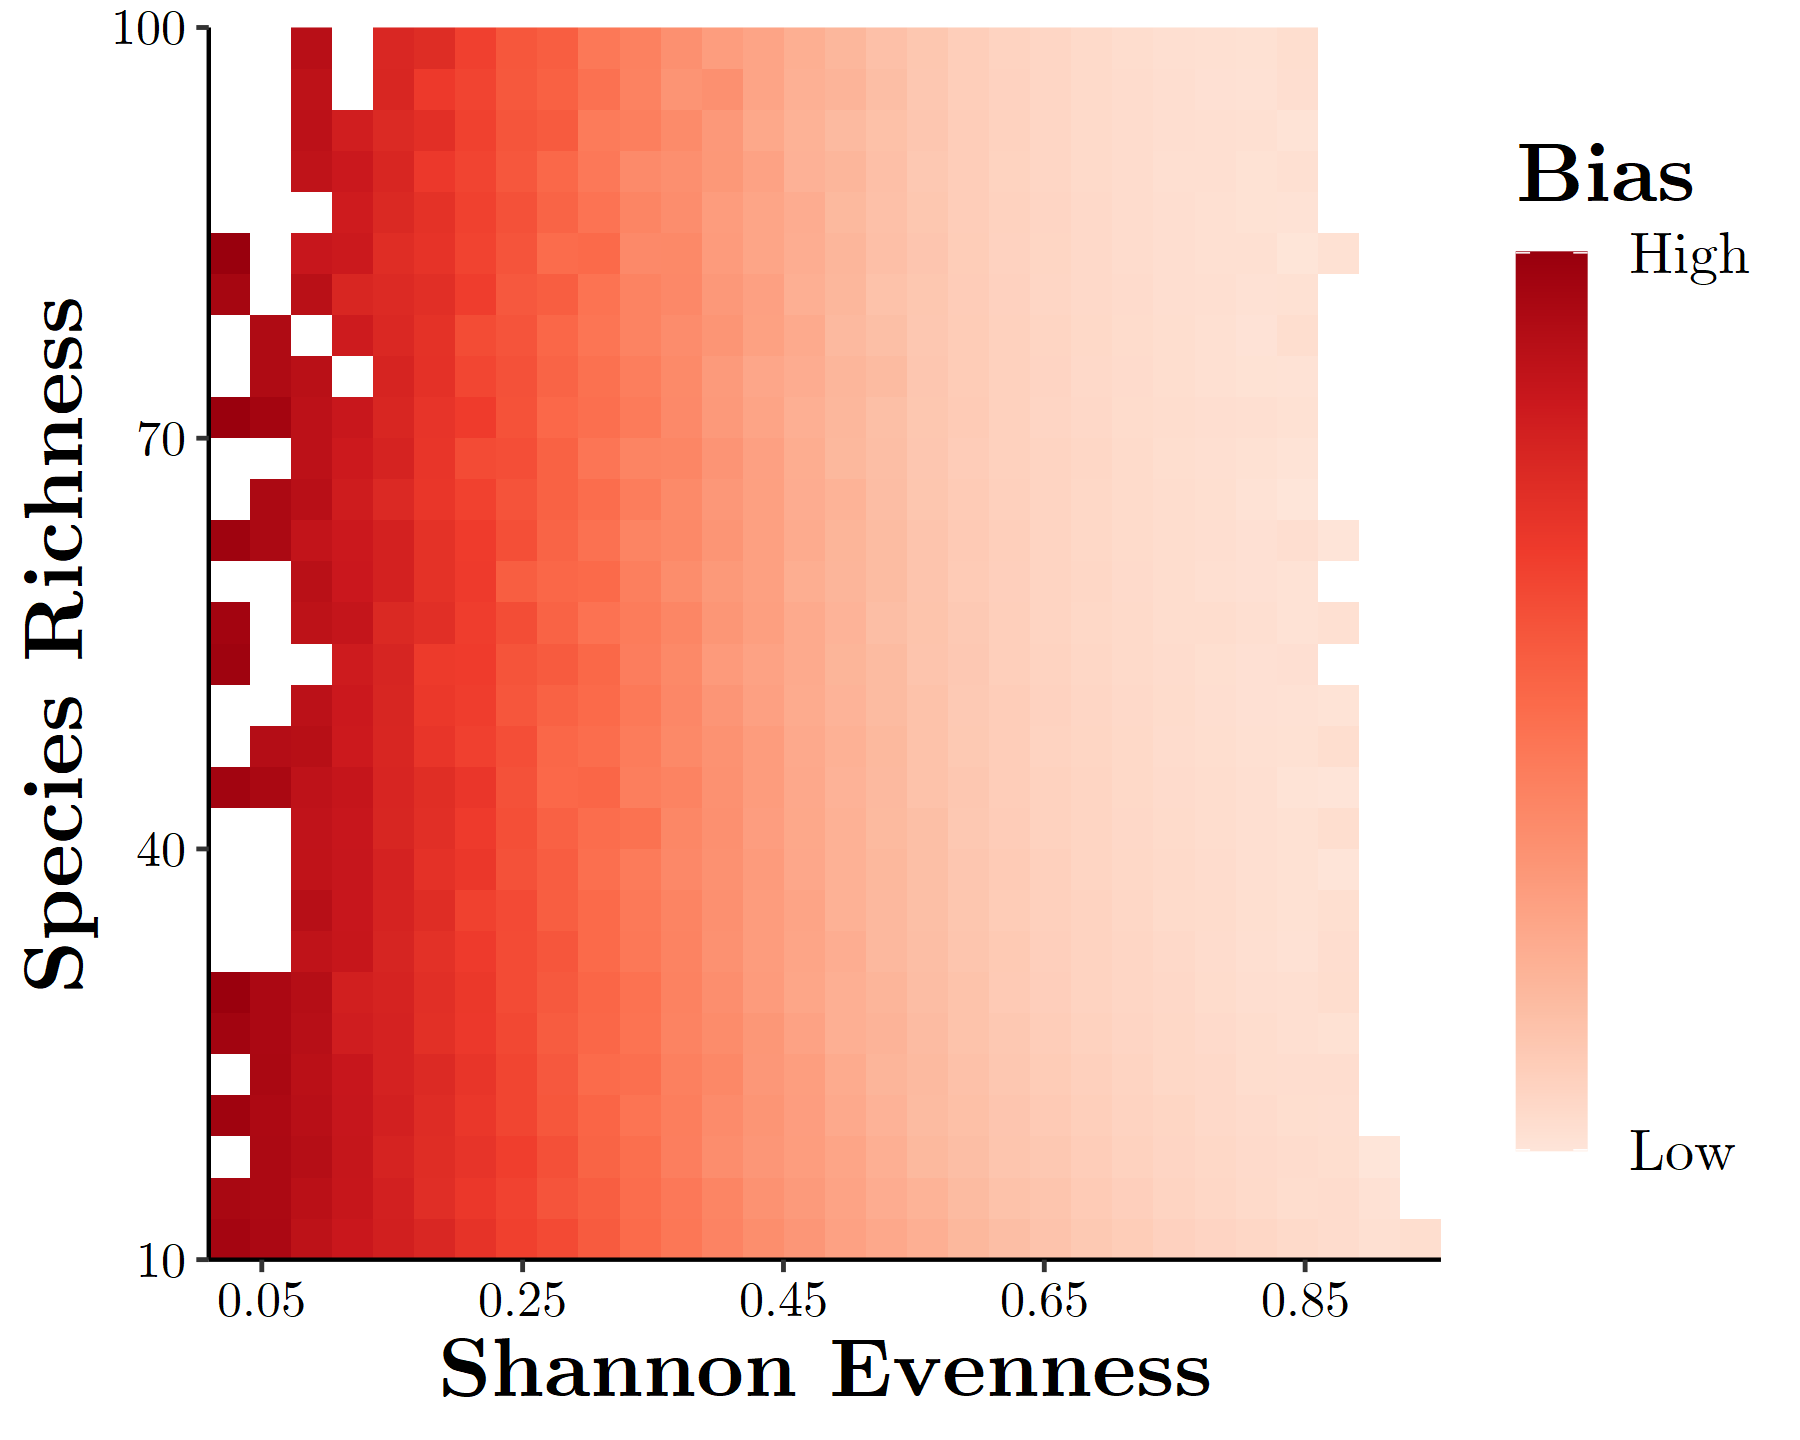
\includegraphics[width=\linewidth]{../Final Visualizations/exampleRandomWeights.png}
  \caption{A baseline for the bias-relationships of functional dispersion. The color is based on an aggregated mean bias, based on 100 000 virtual communities, with log-normal abundance distributions, across 50 evenly spaced values of species richness in $[10,100]$. The log-standard deviation is kept constant at $\sigma_{\log}=2$ \& traits are normally distributed.}
  \label{fig:simFDis}
\end{wrapfigure}

This model framework not only detects, but also decompose the functional index biases into three parts (baseline, species richness, Shannon Evenness). Bias decomposition using this model is done by adding the new components as fixed effects with an interaction with `Type' (the binary parameter indicating the abundance standardization ``treatment''). This addition also allows for interpretation of the unbiased effects of species richness and Shannon Evenness on the functional index at hand. The best fitted models were selected based on the minimum AIC from the set of models that can be constructed by removing fixed effects (see \autoref{ResultsBias}), semi-parametric and random effects were kept the same for all models.

When considering the bias introduced by using presence data instead of abundance data, it is important to consider the conditions under which a bias might arise. For all the functional indices which I analyse in this report, the abundances are used to compute a species-weight vector for each community\textsuperscript{\protect\hyperlink{ref-Villeger2008}{11}}. As such it must be a necessary, but not obviously sufficient, condition, that the abundance composition of communities must be uneven (see \autoref{fig:counterExample}). By considering the following expressions for Shannon diversity given presence (\(\mathrm{D_{Shannon}}(w^\star)\):
\begin{align*}
\mathrm{D_{Shannon}}(w^\star) &= -\mathlarger\sum_{i = 1}^N \frac{w^\star_i}{\Sigma w^\star} \cdot \log\left(\frac{w^\star_i}{\Sigma w^\star}\right), \quad w^\star_i = 
  \begin{dcases}
    1,\quad  w_i > 0 \\ 
    0, \quad w_i = 0 
  \end{dcases} \\
&= -\Sigma w^\star \cdot \frac{1}{\Sigma w^\star} \cdot \log\left(\frac{1}{\Sigma w^\star}\right) = \log(\Sigma w^\star)
\end{align*}
then recognizing \(\Sigma w^\star\) as the number of species present \(N^*\):
\[\mathrm{D_{Shannon}}(w^\star)=\log(N^\star)\]
It becomes clear that Shannon evenness which is defined as\textsuperscript{\protect\hyperlink{ref-Magurran2010}{35}} \(\mathrm{E_{Shannon}} = \frac{\mathrm{D_{Shannon}}(w)}{\log(N)}\), can be reformulated as the ratio between Shannon diversity of a community given abundance data and the same community given presence data:
\[\mathrm{E_{Shannon}}=\frac{\mathrm{D_{Shannon}}(w)}{\mathrm{D_{Shannon}}(w^*)}\]
Thus functional indices for abundance and presence data must converge, when Shannon evenness is equal to 1. For this reason I propose that Shannon evenness can be used as an indicator of possible biases in functional analyses. Simulations also provide a strong expectation that it is indeed Shannon evenness, not species richness, which primarily drives the bias, at least for functional dispersion, see \autoref{fig:simFDis}. However for the data distribution of the real woody plant communities in my investigation, we do not have such broad coverage of Shannon evenness for the entire range of species richness, especially within specific sampling regimes.

\hypertarget{software}{%
\subsection{Software}\label{software}}

All analyses and illustrations were carried out in R (R version 4.1.3 (2022-03-10))\textsuperscript{\protect\hyperlink{ref-R-base}{36}}. Calculation of the functional indices were done using a package I created for the specific purposes and needs of this work, and is accessible on \href{https://github.com/asgersvenning/bachelor}{github (https://github.com/asgersvenning/bachelor)}. The package provides separate functions for calculating the individual indices, as well as support for both euclidean distance and (weighted) Gower dissimilarity, as well as ordination. The package also includes all the data necessary to reproduce my results. It is inspired by the FD\textsuperscript{\protect\hyperlink{ref-R-FD-2}{37}} package, but has some key changes/improvements that allow more flexibility over FD, as well as being faster in some cases. In the backend the package relies heavily on the use of the tidyverse\textsuperscript{\protect\hyperlink{ref-R-tidyverse}{38}} (for data manipulation) and the geometry\textsuperscript{\protect\hyperlink{ref-R-geometry}{39}} package (for computing convex hulls and hypervolumes).

All modelling was done using the GAMM4\textsuperscript{\protect\hyperlink{ref-R-gamm4}{34}} package, which is an extension to the mgcv\textsuperscript{\protect\hyperlink{ref-R-mgcv-5}{33},\protect\hyperlink{ref-R-mgcv-1}{40}--\protect\hyperlink{ref-R-mgcv-4}{43}} package providing more efficient generalized additive mixed models for large numbers of random effects, while classification using Support Vector Machines was done using the kernlab\textsuperscript{\protect\hyperlink{ref-R-kernlab-1}{44},\protect\hyperlink{ref-R-kernlab-2}{45}} package. Visualizations were done using a multitude of packages including but not limited to ggplot2\textsuperscript{\protect\hyperlink{ref-R-ggplot2}{46}}, patchwork\textsuperscript{\protect\hyperlink{ref-R-patchwork}{47}} and sf\textsuperscript{\protect\hyperlink{ref-R-sf}{48}}, while geospatial operations were done using terra\textsuperscript{\protect\hyperlink{ref-R-terra}{49}}, sf\textsuperscript{\protect\hyperlink{ref-R-sf}{48}} and stars\textsuperscript{\protect\hyperlink{ref-R-stars}{50}}. I also thank the creators of the packages hash\textsuperscript{\protect\hyperlink{ref-R-hash}{51}} and magrittr\textsuperscript{\protect\hyperlink{ref-R-magrittr}{52}} for providing cleaner and faster workflows. Scripts for visualizations and analyses will be available on the package github.

\newpage

\hypertarget{results}{%
\section{Results}\label{results}}

\hypertarget{mapSection}{%
\subsection{Spatio-topological patterns of functional space}\label{mapSection}}

The most obvious spatio-topological pattern in the functional space is a clear distinction between the eastern and western United States as can be seen in \autoref{fig:indicesByEcoregion} \& \autoref{fig:interpolatedMaps}. The east-west divide is also visible in the distribution of topological patterns across ecoregions, however, several ecoregions diverge from this pattern, notably the Everglades in Florida. It is also striking that FDis and FEve are consistently larger using presence data, while FDiv is basically unchanged across different ecosystems. All three indices (FDis, FDiv, FEve) also show smaller variance under presence than abundance.

\begin{figure}
  \centering
  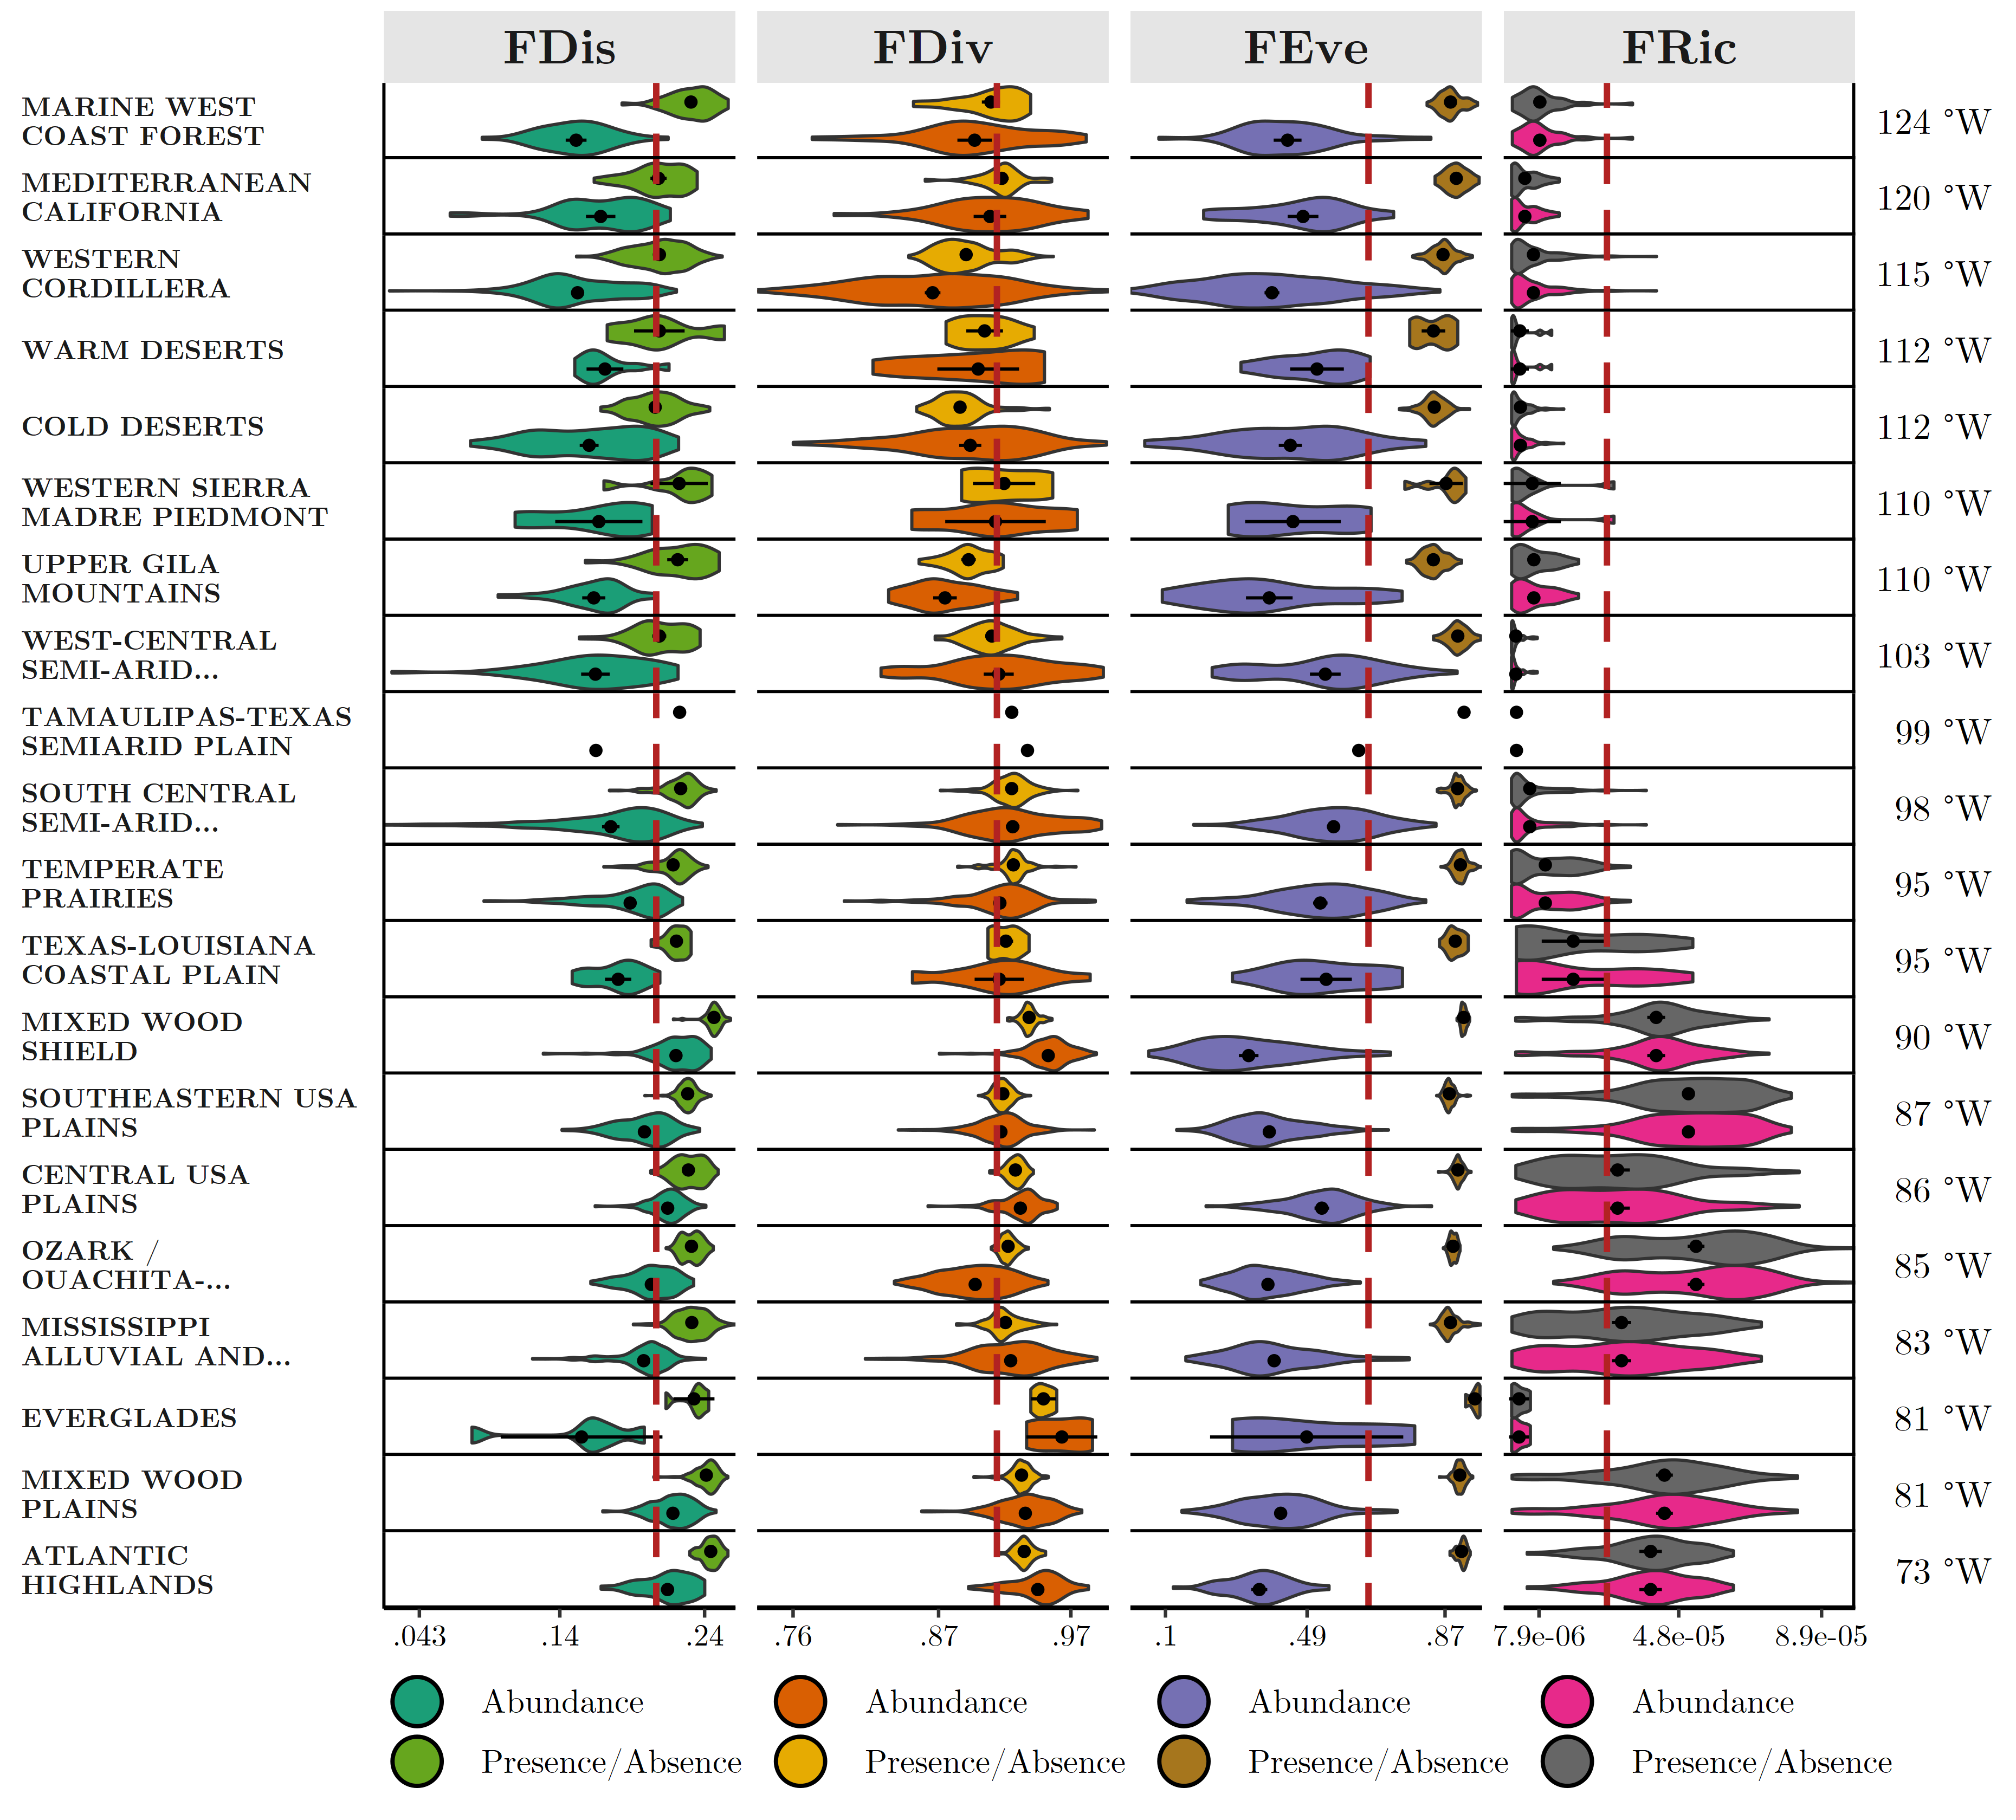
\includegraphics[width=\textwidth]{../Final Visualizations/index_by_ecoregion.png}
  \caption{Functional indices disaggregated by ecoregion arranged: West (top) to East (bottom). The dashed red line indicates the overall mean for each index, while the horizontal black error bars indicate 95\% confidence intervals. Coordinates on the right vertical axis annotate the approximate centroid longitude of each Ecoregion.}
  \label{fig:indicesByEcoregion}
  \vspace{-3cm}     
\end{figure}

\newpage

\begin{figure}
  \centering
  \includegraphics[width=\textwidth]{../Final Visualizations/interpolatedMap.png}
  \caption{Interpolated spatial patterns in the topological indices of the functional ecological space. The values for the functional indices (FDis: \textbf{(a.*)}, FDiv = \textbf{(b.*)}, FEve = \textbf{(c.*)}, FRic = \textbf{(d.*)}) are calculated using the relative weighted mean abundances of species (panel \textbf{(*.1)}) and presence values (panel \textbf{(*.2)}). Grid cells with too species (n$<7$) are interpolated using local distance-weighted geographic regression. The raw maps can be found in \aref{appendixMaps}.}
  \label{fig:interpolatedMaps}
\end{figure}

\FloatBarrier

\newpage

\hypertarget{ResultsBias}{%
\subsection{Biases in functional analysis using presence}\label{ResultsBias}}

\newlength{\oldintextsep}
\setlength{\oldintextsep}{\intextsep}

\setlength{\intextsep}{0pt}
\begin{wraptable}{l}{0pt}

\centering
\begin{tabular}[t]{rccr}
\toprule
  & Sum Sq & F value & Pr(>F)\\
\midrule
\addlinespace[0.3em]
\multicolumn{4}{l}{\textbf{FDis}}\\
\rule{0pt}{2.2ex}\hspace{1em}\cellcolor{gray!6}{With} & \cellcolor{gray!6}{0.045} & \cellcolor{gray!6}{5.953} & \cellcolor{gray!6}{$0.0150\star $}\\
[0.2ex]
\rule{0pt}{2.2ex}\hspace{1em}Without & 0.300 & 36.530 & $2.9 \cdot 10^{-09}\star \star \star $\\
[0.2ex]
\addlinespace[0.3em]
\multicolumn{4}{l}{\textbf{FDiv}}\\
\rule{0pt}{2.2ex}\hspace{1em}\cellcolor{gray!6}{With} & \cellcolor{gray!6}{$1.4 \cdot 10^{-04}$} & \cellcolor{gray!6}{0.029} & \cellcolor{gray!6}{$0.8636$}\\
[0.2ex]
\rule{0pt}{2.2ex}\hspace{1em}Without & $3.4 \cdot 10^{-05}$ & 0.007 & $0.9316$\\
[0.2ex]
\addlinespace[0.3em]
\multicolumn{4}{l}{\textbf{FEve}}\\
\rule{0pt}{2.2ex}\hspace{1em}\cellcolor{gray!6}{With} & \cellcolor{gray!6}{$4.2 \cdot 10^{-04}$} & \cellcolor{gray!6}{0.141} & \cellcolor{gray!6}{$0.7068$}\\
[0.2ex]
\rule{0pt}{2.2ex}\hspace{1em}Without & 0.011 & 3.666 & $0.0560.$\\
[0.2ex]
\bottomrule
\end{tabular}
\caption{\label{tab:simTab}ANOVA type 2 results (simulated data) for the effect of species richness on functional indices with and without Shannon evenness included.}

\vspace{0.7cm}
\end{wraptable}

In the woody plant assemblages I investigated, the variance (and to some degree mean) of Shannon Evenness is strongly correlated with species richness, particularly in the low to medium sampling density regime (0-200 plots). To illustrate the issues that might arise from this structure I ran a simulation across the three topological functional indices which integrate abundances, with species richness in the range 10-100 following a log-normal abundance distributed communities (\(\mu_{\log}=-4,\quad\sigma_{\log}=1.25\)) with 5 uniformly distributed traits for each virtual species\footnote{The distribution parameters are chosen to mimic the ones in the FIA dataset.}. I then ran a set of type II ANOVA's on linear models of the bias (for each index) using either only species richness, or species richness along with Shannon evenness. This synthetic analysis shows how a correlation structure between species richness and unknown true predictors of bias (Shannon Evenness), can result in potentially misleading findings (\autoref{tab:simTab}).

\begin{table}[!h]

\vspace{.25cm}
\centering
\begin{threeparttable}
\begin{tabular}[t]{lcccr}
\toprule
  & Estimate & Std. Error & t value & Pr(>|t|)\\
\midrule
\addlinespace[0.3em]
\multicolumn{1}{l}{\textbf{FDis}}\\
\rule{0pt}{2.75ex}\hspace{1em}\cellcolor{gray!6}{$\beta$} & \cellcolor{gray!6}{0.189} & \cellcolor{gray!6}{0.001} & \cellcolor{gray!6}{170.005} & \cellcolor{gray!6}{$0\star \star \star $}\\
[0.75ex]
\rule{0pt}{2.75ex}\hspace{1em}$\beta^\mathrm{Bias}$ & 0.036 & $2.6 \cdot 10^{-04}$ & 140.861 & $0\star \star \star $\\
[0.75ex]
\rule{0pt}{2.75ex}\hspace{1em}\cellcolor{gray!6}{$\alpha_{\mathrm{Richness}}$} & \cellcolor{gray!6}{0.020} & \cellcolor{gray!6}{0.001} & \cellcolor{gray!6}{19.165} & \cellcolor{gray!6}{$1.1 \cdot 10^{-78}\star \star \star $}\\
[0.75ex]
\rule{0pt}{2.75ex}\hspace{1em}$\alpha_{\mathrm{Shannon\,Evenness}}$ & 0.020 & $3.2 \cdot 10^{-04}$ & 63.220 & $0\star \star \star $\\
[0.75ex]
\rule{0pt}{2.75ex}\hspace{1em}\cellcolor{gray!6}{$\alpha^{\mathrm{Bias}}_{\mathrm{Richness}}$} & \cellcolor{gray!6}{-0.003} & \cellcolor{gray!6}{0.001} & \cellcolor{gray!6}{-2.901} & \cellcolor{gray!6}{$0.0037\star \star $}\\
[0.75ex]
\rule{0pt}{2.75ex}\hspace{1em}$\alpha^{\mathrm{Bias}}_{\mathrm{Shannon\,Evenness}}$ & -0.021 & $3.8 \cdot 10^{-04}$ & -57.427 & $0\star \star \star $\\
[0.75ex]
\addlinespace[0.3em]
\multicolumn{1}{l}{\textbf{FDiv}}\\
\rule{0pt}{2.75ex}\hspace{1em}\cellcolor{gray!6}{$\beta$} & \cellcolor{gray!6}{0.911} & \cellcolor{gray!6}{0.001} & \cellcolor{gray!6}{859.329} & \cellcolor{gray!6}{$0\star \star \star $}\\
[0.75ex]
\rule{0pt}{2.75ex}\hspace{1em}$\beta^\mathrm{Bias}$ & 0.005 & $5.2 \cdot 10^{-04}$ & 10.220 & $3 \cdot 10^{-24}\star \star \star $\\
[0.75ex]
\addlinespace[0.3em]
\multicolumn{1}{l}{\textbf{FEve}}\\
\rule{0pt}{2.75ex}\hspace{1em}\cellcolor{gray!6}{$\beta$} & \cellcolor{gray!6}{0.429} & \cellcolor{gray!6}{0.001} & \cellcolor{gray!6}{251.252} & \cellcolor{gray!6}{$0\star \star \star $}\\
[0.75ex]
\rule{0pt}{2.75ex}\hspace{1em}$\beta^\mathrm{Bias}$ & 0.459 & 0.002 & 190.751 & $0\star \star \star $\\
[0.75ex]
\rule{0pt}{2.75ex}\hspace{1em}\cellcolor{gray!6}{$\alpha_{\mathrm{Shannon\,Evenness}}$} & \cellcolor{gray!6}{0.021} & \cellcolor{gray!6}{0.002} & \cellcolor{gray!6}{9.133} & \cellcolor{gray!6}{$9.8 \cdot 10^{-20}\star \star \star $}\\
[0.75ex]
\rule{0pt}{2.75ex}\hspace{1em}$\alpha^{\mathrm{Bias}}_{\mathrm{Shannon\,Evenness}}$ & -0.024 & 0.003 & -7.529 & $6.1 \cdot 10^{-14}\star \star \star $\\
[0.75ex]
\bottomrule
\end{tabular}
\caption{\label{tab:realTab}Summary statistics for the best models (real data) selected based on minimi-zing AIC. Predictors are scaled (after transformation).}

\end{threeparttable}
\vspace{1cm}
\end{table}

Using the abundances from FIA and traits from PLANTS, I found a significant positive bias for all three functional indices which can integrate abundance (FDis, FDiv and FEve), using a generalized additive mixed model (GAMM) adjusting for both spatial and sampling patterns, as well as differences between ecosystems. This result falls in line with the visual patterns found in \autoref{mapSection} (see \autoref{fig:indicesByEcoregion}). This bias was decomposed by expanding the fixed effects, \(X\boldsymbol{\beta}\), in the GAMM model as follows:
\begin{align*}
  X\boldsymbol{\beta}&=\beta + \alpha_\mathrm{Richness}\cdot\mathrm{Richness} + \alpha_\mathrm{Shannon\,Evenness}\cdot\mathrm{Shannon\,Evenness} + \mathbf{B} \\
  \mathbf{B}&=T\cdot(\beta^\mathrm{Bias} + \alpha^\mathrm{Bias}_\mathrm{Richness} + \alpha^\mathrm{Bias}_\mathrm{Shannon\,Evenness}\cdot\mathrm{Shannon\,Evenness})
\end{align*}
Where \(T\) is short for data standardization \textbf{T}ype and is an indicator variable which is equal to 1, when the data is presence-only. The first three parameters (\(\beta,\,\alpha_\mathrm{Richness},\,\alpha_\mathrm{Shannon\,Evenness}\)) model the patterns in the values of the index given abundance data, while the latter three parameters in \(\mathbf{B}\) model the difference (bias) in the value of the index given presence data. The decomposition of \(\mathbf{B}\) can be interpreted as the estimated\ldots:

\begin{enumerate}
  \itemsep0em 
  \item[-] $\beta$: functional index value using abundances given the mean of the transformed predictors.
  \item[-] $\alpha_\mathrm{Richness}$: scaled log-linear relationship between species richness and the functional index given abundances.
  \item[-] $\alpha_\mathrm{Shannon\,Evenness}$: scaled linear relationship between Shannon Evenness and the functional index given abundances.
  \item[-] $\beta^\mathrm{Bias}$: baseline bias component given presence data.
  \item[-] $\alpha^\mathrm{Bias}_\mathrm{Richness}$: scaled log-linear bias component explained by species richness given presence data.
  \item[-] $\alpha^\mathrm{Bias}_\mathrm{Shannon\,Evenness}$: scaled linear bias component explained by Shannon Evenness given presence data.
\end{enumerate}

As expected for the indices with a significant bias (FDis and FEve), the estimated component for Shannon Evenness, \(\alpha^\mathrm{Bias}_\mathrm{Shannon\,Evenness}\), is highly significant and large in magnitude, while the estimated component for species richness, \(\alpha^\mathrm{Bias}_\mathrm{Richness}\), is smaller in magnitude and/or insignificant, as can be seen in \autoref{tab:realTab}. For FDiv only the baseline bias component was even slightly significant based on model AIC, however the variance in FDiv was much smaller given presence data (not shown).

\setlength{\intextsep}{\oldintextsep}

\begin{figure}
  \centering
  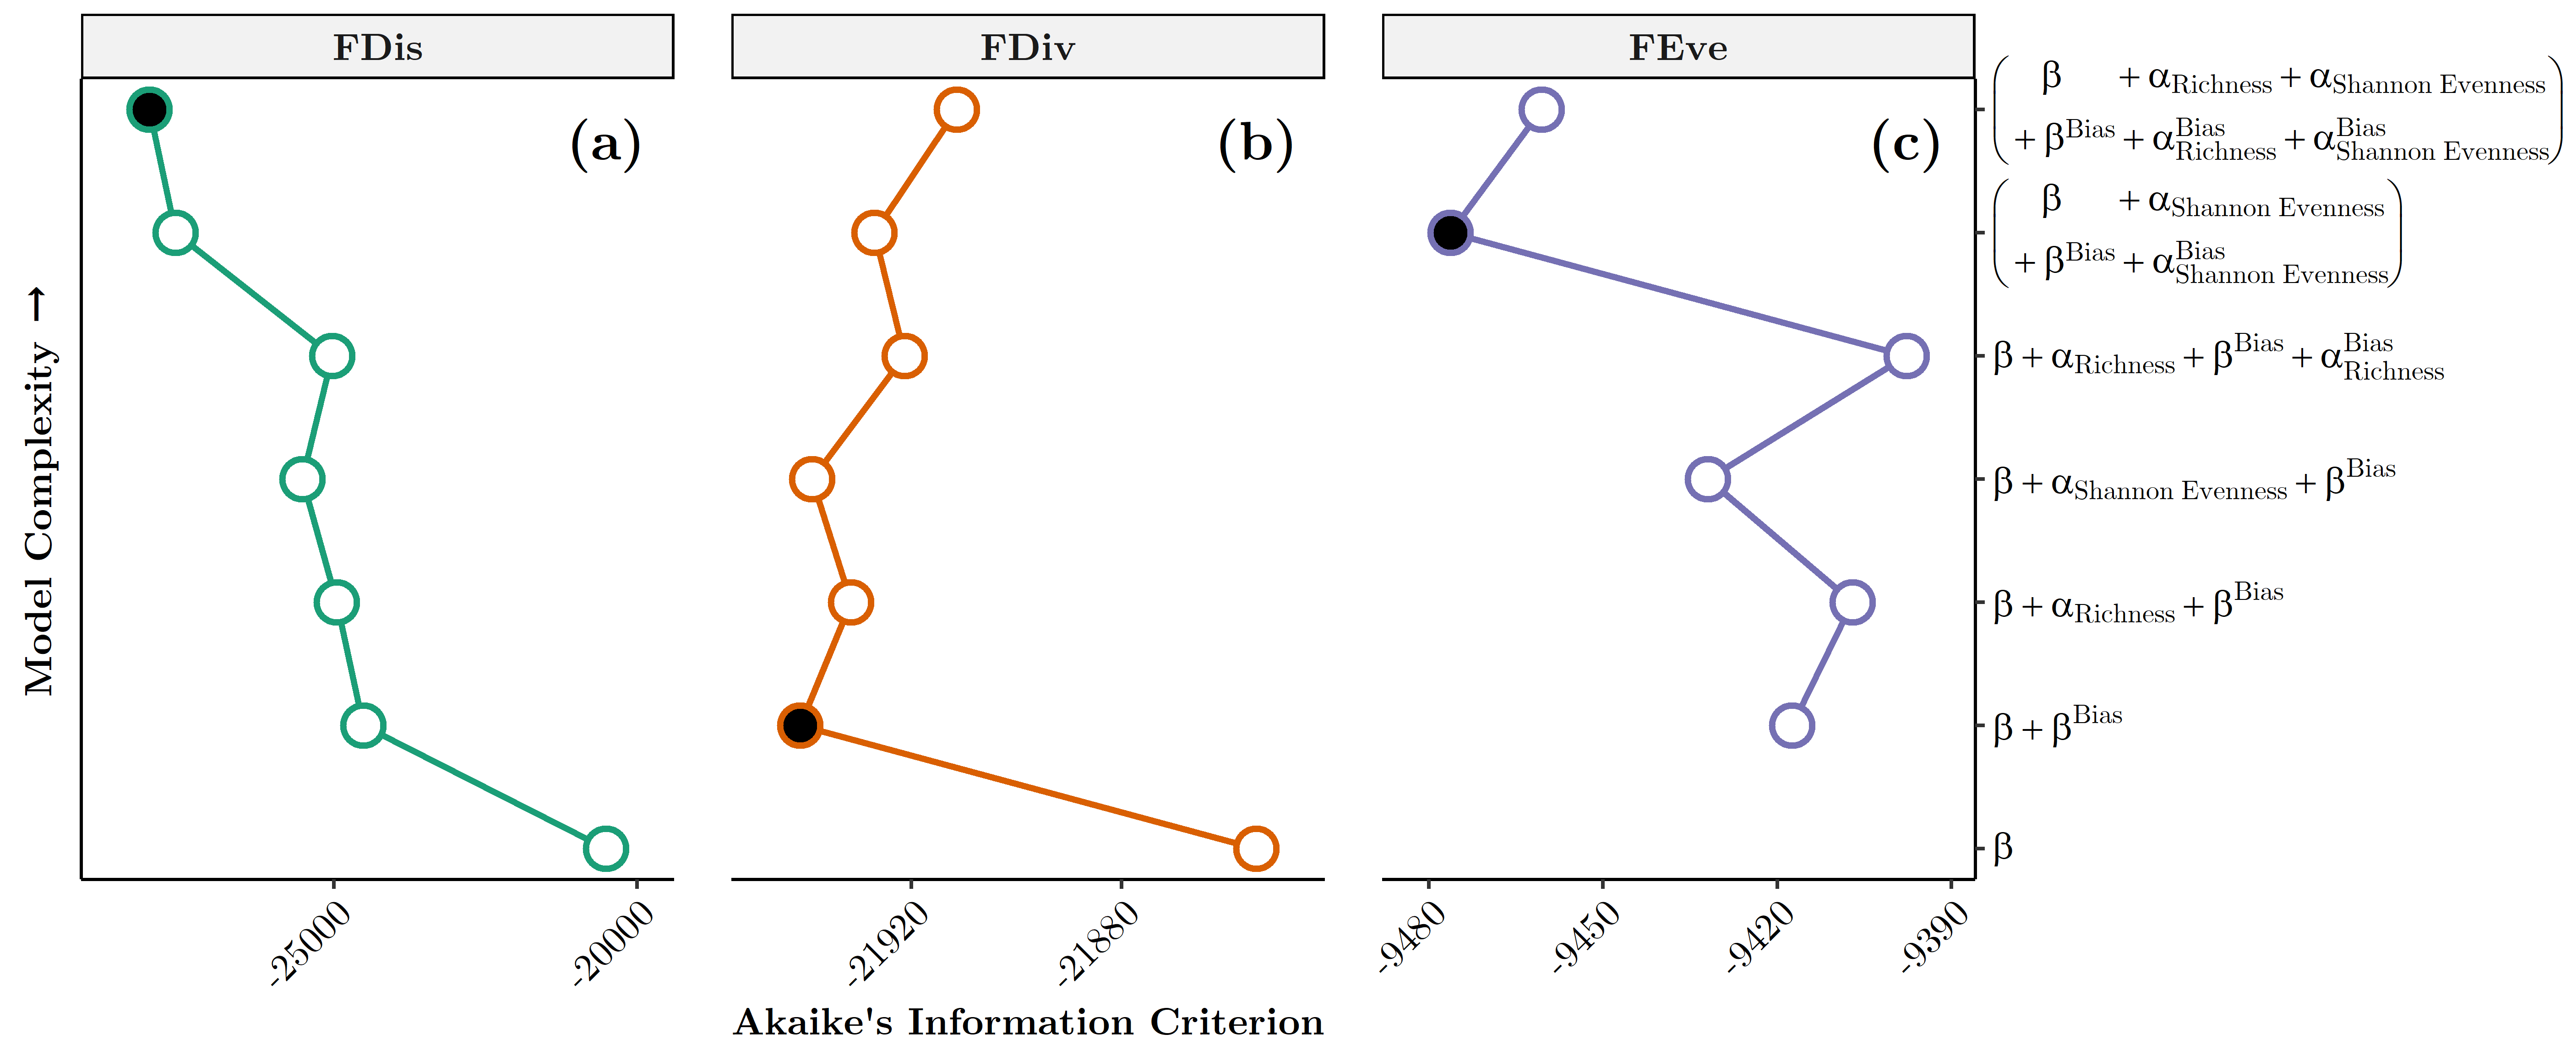
\includegraphics[width=\textwidth]{../Final Visualizations/finalModelAIC.png}
  \caption{Model selection based on minimizing AIC. The intercept only model for FEve \textbf{(c)} is not shown due to extreme AIC (AIC = 335).}
  \label{fig:modelAIC}
\end{figure}

\hypertarget{discussion}{%
\section{Discussion}\label{discussion}}

Here I have shown the functional indices FDis and especially FEve, are biased when presence data is used, and that this bias is strongly related to the evenness of the abundance distribution. This is not entirely surprising and makes sense ecologically, given that communities where the abundance is mainly concentrated on a few species, will likely be less functionally diverse than communities where abundance is spread more evenly among species, which is inherently assumed in presence data.

Although the effects of integrating abundances seem to suggest that limiting similarity is less important than what is traditionally thought, the species richness relationships that I find support the theory of carrying capacity of species richness\textsuperscript{\protect\hyperlink{ref-Storch2019}{3}}. Both functional divergence and evenness show no significant correlation with species richness. Thus, clustering of species in functional space is also not correlated with species richness, suggesting that niche partitioning occurs equally at all levels of species richness supporting the theory of limiting similarity. However the most significant species richness relationship that I find, is a positive correlation with functional dispersion suggesting that niche partitioning begins at the central niche in a community, which I hypothesize is often most productive. If true, this pattern can be explained by species richness-productivity relationships which have been shown associated with niche packing\textsuperscript{\protect\hyperlink{ref-Pellissier2018}{53}}. My results thus show that species-rich communities are more functionally diverse, even and show increasing partitioning of the niche space. These patterns are initially strongly correlated with the sampling regime, which is especially evident in the spatial patterns of the functional indices, however the reported relationships are adjusted for spatial, ecosystem and sampling effects.

I interpret the strong longitudinal divide as a coupled ecological and sampling effect. There are clearly different sampling regimes in the eastern and western parts of FIA effort\textsuperscript{\protect\hyperlink{ref-Mcroberts2005}{54},\protect\hyperlink{ref-Wiener2021}{55}} (also see \aref{appendixSampling}), however at the same time the western United States is covered by large swathes of deserts, which might be unsuitable for the FIA, and coniferous forests which show different patterns of functional diversity compared to decidous forests\textsuperscript{\protect\hyperlink{ref-Lubek2020}{56}}.

A caveat to the rigor of this model, is a large degree of residual heteroscedacity between abundances and presence, with abundances generally displaying much larger variance. I was unfortunately not able to resolve this due to the gamm4 package not supporting general model classes (in this case the ``gaulss'' family, would be more appropriate) while the alternative solution using random effects in gam (from the package mgcv) is exceedingly slow when the number of random effects is large (in this case n = 2291). The effect of this compromise is likely larger standard errors (higher p-values) on the estimated effects given abundances, and likewise smaller standard errors (lower p-values) for the estimated effects given presence.

\hypertarget{summary}{%
\section{Summary}\label{summary}}

I find significant biases in certain functional indicies (FDis, FEve) when comparing presence data with abundance data underscoring the need for greater integration of abundances in functional ecology, a trend which I expect will happen naturally, as data availability and statistical/modelling knowledge increases. This work also provides further support for the carrying capacity of species richness\textsuperscript{\protect\hyperlink{ref-Storch2019}{3}} and limiting similarity, by showing that species-rich areas are not more functionally clustered. Future work on robust testing of these patterns using abundance permutation tests on multiple spatial scales and extending the work beyond the US and woody plants is needed however, before we can be fully confident in the patterns I have shown here and their ecological generality.

\newpage

\hypertarget{references}{%
\section{References}\label{references}}

\hypertarget{refs}{}
\begin{CSLReferences}{0}{0}
\leavevmode\vadjust pre{\hypertarget{ref-IPBES2019}{}}%
\CSLLeftMargin{1. }
\CSLRightInline{IPBES. {Global assessment report on biodiversity and ecosystem services of the Intergovernmental Science-Policy Platform on Biodiversity and Ecosystem Services}. (2019) doi:\href{https://doi.org/10.5281/ZENODO.6417333}{10.5281/ZENODO.6417333}.}

\leavevmode\vadjust pre{\hypertarget{ref-Lavorel2002}{}}%
\CSLLeftMargin{2. }
\CSLRightInline{Lavorel, S. \& Garnier, E. \href{https://doi.org/10.1046/J.1365-2435.2002.00664.X}{{Predicting changes in community composition and ecosystem functioning from plant traits: revisiting the Holy Grail}}. \emph{Functional Ecology} \textbf{16}, 545--556 (2002).}

\leavevmode\vadjust pre{\hypertarget{ref-Storch2019}{}}%
\CSLLeftMargin{3. }
\CSLRightInline{Storch, D. \& Okie, J. G. \href{https://doi.org/10.1111/geb.12987}{{The carrying capacity for species richness}}. \emph{Global Ecology and Biogeography} \textbf{28}, 1519--1532 (2019).}

\leavevmode\vadjust pre{\hypertarget{ref-Rabosky2015}{}}%
\CSLLeftMargin{4. }
\CSLRightInline{Rabosky, D. L. \& Hurlbert, A. H. \href{https://doi.org/10.1086/680850/ASSET/IMAGES/LARGE/FG3.JPEG}{{Species richness at continental scales is dominated by ecological limits}}. \emph{American Naturalist} \textbf{185}, 572--583 (2015).}

\leavevmode\vadjust pre{\hypertarget{ref-Ricklefs2012}{}}%
\CSLLeftMargin{5. }
\CSLRightInline{Ricklefs, R. E. \href{https://doi.org/10.1073/pnas.1212079109}{{Species richness and morphological diversity of passerine birds}}. \emph{Proceedings of the National Academy of Sciences} \textbf{109}, 14482 LP--14487 (2012).}

\leavevmode\vadjust pre{\hypertarget{ref-Mouillot2013}{}}%
\CSLLeftMargin{6. }
\CSLRightInline{Mouillot, D., Graham, N. A. J., Villéger, S., Mason, N. W. H. \& Bellwood, D. R. \href{https://doi.org/10.1016/j.tree.2012.10.004}{{A functional approach reveals community responses to disturbances}}. \emph{Trends in Ecology \& Evolution} \textbf{28}, 167--177 (2013).}

\leavevmode\vadjust pre{\hypertarget{ref-Swenson2016}{}}%
\CSLLeftMargin{7. }
\CSLRightInline{Swenson, N. G. \emph{et al.} \href{https://doi.org/10.1086/685083}{{Constancy in Functional Space across a Species Richness Anomaly}}. \emph{The American Naturalist} \textbf{187}, E83--E92 (2016).}

\leavevmode\vadjust pre{\hypertarget{ref-Ordonez2018}{}}%
\CSLLeftMargin{8. }
\CSLRightInline{Ordonez, A. \& Svenning, J. C. \href{https://doi.org/10.1111/geb.12785}{{Greater tree species richness in eastern North America compared to Europe is coupled to denser, more clustered functional trait space filling, not to trait space expansion}}. \emph{Global Ecology and Biogeography} \textbf{27}, 1288--1299 (2018).}

\leavevmode\vadjust pre{\hypertarget{ref-McGill2006}{}}%
\CSLLeftMargin{9. }
\CSLRightInline{McGill, B. J., Enquist, B. J., Weiher, E. \& Westoby, M. \href{https://doi.org/10.1016/J.TREE.2006.02.002}{{Rebuilding community ecology from functional traits}}. \emph{Trends in Ecology and Evolution} \textbf{21}, 178--185 (2006).}

\leavevmode\vadjust pre{\hypertarget{ref-Paine2015}{}}%
\CSLLeftMargin{10. }
\CSLRightInline{Paine, C. E. T. \emph{et al.} \href{https://doi.org/10.1111/1365-2745.12401}{{Globally, functional traits are weak predictors of juvenile tree growth, and we do not know why}}. \emph{Journal of Ecology} \textbf{103}, 978--989 (2015).}

\leavevmode\vadjust pre{\hypertarget{ref-Villeger2008}{}}%
\CSLLeftMargin{11. }
\CSLRightInline{Villéger, S., Mason, N. W. H. \& Mouillot, D. \href{https://doi.org/10.1890/07-1206.1}{{NEW MULTIDIMENSIONAL FUNCTIONAL DIVERSITY INDICES FOR A MULTIFACETED FRAMEWORK IN FUNCTIONAL ECOLOGY}}. \emph{Ecology} \textbf{89}, 2290--2301 (2008).}

\leavevmode\vadjust pre{\hypertarget{ref-Mouchet2010}{}}%
\CSLLeftMargin{12. }
\CSLRightInline{Mouchet, M. A., Villéger, S., Mason, N. W. H. \& Mouillot, D. \href{https://doi.org/10.1111/j.1365-2435.2010.01695.x}{{Functional diversity measures: an overview of their redundancy and their ability to discriminate community assembly rules}}. \emph{Functional Ecology} \textbf{24}, 867--876 (2010).}

\leavevmode\vadjust pre{\hypertarget{ref-Violle2014}{}}%
\CSLLeftMargin{13. }
\CSLRightInline{Violle, C., Reich, P. B., Pacala, S. W., Enquist, B. J. \& Kattge, J. \href{https://doi.org/10.1073/pnas.1415442111}{{The emergence and promise of functional biogeography}}. \emph{Proceedings of the National Academy of Sciences of the United States of America} \textbf{111}, 13690--13696 (2014).}

\leavevmode\vadjust pre{\hypertarget{ref-Weiher1998}{}}%
\CSLLeftMargin{14. }
\CSLRightInline{Weiher, E., Clarke, G. D. P. \& Keddy, P. A. \href{https://doi.org/10.2307/3547051}{{Community Assembly Rules, Morphological Dispersion, and the Coexistence of Plant Species}}. \emph{Oikos} \textbf{81}, (1998).}

\leavevmode\vadjust pre{\hypertarget{ref-Scherer2008}{}}%
\CSLLeftMargin{15. }
\CSLRightInline{Scherer-Lorenzen, M. \href{https://doi.org/10.1111/J.1365-2435.2008.01389.X}{{Functional diversity affects decomposition processes in experimental grasslands}}. \emph{Functional Ecology} \textbf{22}, 547--555 (2008).}

\leavevmode\vadjust pre{\hypertarget{ref-Zavaleta2010}{}}%
\CSLLeftMargin{16. }
\CSLRightInline{Zavaleta, E. S., Pasari, J. R., Hulvey, K. B. \& Tilman, G. D. \href{https://doi.org/10.1073/PNAS.0906829107}{{Sustaining multiple ecosystem functions in grassland communities requires higher biodiversity}}. \emph{Proceedings of the National Academy of Sciences of the United States of America} \textbf{107}, 1443--1446 (2010).}

\leavevmode\vadjust pre{\hypertarget{ref-Hejda2013}{}}%
\CSLLeftMargin{17. }
\CSLRightInline{Hejda, M. \& Bello, F. de. \href{https://doi.org/10.1111/JVS.12026}{{Impact of plant invasions on functional diversity in the vegetation of Central Europe}}. \emph{Journal of Vegetation Science} \textbf{24}, 890--897 (2013).}

\leavevmode\vadjust pre{\hypertarget{ref-Catford2019}{}}%
\CSLLeftMargin{18. }
\CSLRightInline{Catford, J. A. \emph{et al.} \href{https://doi.org/10.1111/ele.13220}{{Traits linked with species invasiveness and community invasibility vary with time, stage and indicator of invasion in a long-term grassland experiment}}. \emph{Ecology Letters} \textbf{22}, 593--604 (2019).}

\leavevmode\vadjust pre{\hypertarget{ref-Yang2018}{}}%
\CSLLeftMargin{19. }
\CSLRightInline{Yang, J., Cao, M. \& Swenson, N. G. \href{https://doi.org/10.1016/j.tree.2018.03.003}{{Why Functional Traits Do Not Predict Tree Demographic Rates}}. \emph{Trends in Ecology and Evolution} \textbf{33}, 326--336 (2018).}

\leavevmode\vadjust pre{\hypertarget{ref-Svenning2015}{}}%
\CSLLeftMargin{20. }
\CSLRightInline{Svenning, J.-C., Eiserhardt, W. L., Normand, S., Ordonez, A. \& Sandel, B. \href{https://doi.org/10.1146/annurev-ecolsys-112414-054314}{{The Influence of Paleoclimate on Present-Day Patterns in Biodiversity and Ecosystems}}. \emph{Annu. Rev. Ecol. Evol. Syst} \textbf{46}, 551--72 (2015).}

\leavevmode\vadjust pre{\hypertarget{ref-Culshaw2021}{}}%
\CSLLeftMargin{21. }
\CSLRightInline{Culshaw, V., Mairal, M. \& Sanmartín, I. \href{https://doi.org/10.3389/FEVO.2021.662092/BIBTEX}{{Biogeography Meets Niche Modeling: Inferring the Role of Deep Time Climate Change When Data Is Limited}}. \emph{Frontiers in Ecology and Evolution} \textbf{9}, 599 (2021).}

\leavevmode\vadjust pre{\hypertarget{ref-Swenson2010}{}}%
\CSLLeftMargin{22. }
\CSLRightInline{Swenson, N. G. \& Weiser, M. D. \href{https://doi.org/10.1890/09-1743.1}{{Plant geography upon the basis of functional traits: An example from eastern North American trees}}. \emph{Ecology} \textbf{91}, 2234--2241 (2010).}

\leavevmode\vadjust pre{\hypertarget{ref-Swenson2012}{}}%
\CSLLeftMargin{23. }
\CSLRightInline{Swenson, N. G. \emph{et al.} \href{https://doi.org/10.1111/J.1466-8238.2011.00727.X}{{The biogeography and filtering of woody plant functional diversity in North and South America}}. \emph{Global Ecology and Biogeography} \textbf{21}, 798--808 (2012).}

\leavevmode\vadjust pre{\hypertarget{ref-Blonder2018}{}}%
\CSLLeftMargin{24. }
\CSLRightInline{Blonder, B. \emph{et al.} \href{https://doi.org/10.1111/GCB.14375}{{Late Quaternary climate legacies in contemporary plant functional composition}}. \emph{Global Change Biology} \textbf{24}, 4827--4840 (2018).}

\leavevmode\vadjust pre{\hypertarget{ref-FIADB}{}}%
\CSLLeftMargin{25. }
\CSLRightInline{U.S. Department of Agriculture, Forest Service, N. R. S. \href{https://apps.fs.usda.gov/fia/datamart/CSV/datamart_csv.html}{{Forest Inventory and Analysis Database}}. (2022).}

\leavevmode\vadjust pre{\hypertarget{ref-sauer2008north}{}}%
\CSLLeftMargin{26. }
\CSLRightInline{Sauer, J. R., Hines, J. E. \& Fallon, J. {The North American breeding bird survey, results and analysis 1966--2007. Version 5.15. 2008}. \emph{US geological Survey Patuxent Wildlife research center, laurel, maryland} (2008).}

\leavevmode\vadjust pre{\hypertarget{ref-Gillings2019}{}}%
\CSLLeftMargin{27. }
\CSLRightInline{Gillings, S. \emph{et al.} \href{https://doi.org/10.1111/GEB.12906}{{Breeding and wintering bird distributions in Britain and Ireland from citizen science bird atlases}}. \emph{Global Ecology and Biogeography} \textbf{28}, 866--874 (2019).}

\leavevmode\vadjust pre{\hypertarget{ref-PLANTS}{}}%
\CSLLeftMargin{28. }
\CSLRightInline{USDA, N. \emph{{The PLANTS Database}}. \url{http://plants.usda.gov} (2022).}

\leavevmode\vadjust pre{\hypertarget{ref-Fraser2020}{}}%
\CSLLeftMargin{29. }
\CSLRightInline{Fraser, L. H. \href{https://doi.org/10.1111/GCB.14869}{{TRY---A plant trait database of databases}}. \emph{Global Change Biology} \textbf{26}, 189--190 (2020).}

\leavevmode\vadjust pre{\hypertarget{ref-Wilman2014}{}}%
\CSLLeftMargin{30. }
\CSLRightInline{Wilman, H. \emph{et al.} \href{https://doi.org/10.1890/13-1917.1}{{EltonTraits 1.0: Species-level foraging attributes of the world's birds and mammals}}. \emph{Ecology} \textbf{95}, 2027--2027 (2014).}

\leavevmode\vadjust pre{\hypertarget{ref-Laliberte2010}{}}%
\CSLLeftMargin{31. }
\CSLRightInline{Laliberté, E. \& Legendre, P. \href{https://doi.org/10.1890/08-2244.1}{{A distance-based framework for measuring functional diversity from multiple traits}}. \emph{Ecology} \textbf{91}, 299--305 (2010).}

\leavevmode\vadjust pre{\hypertarget{ref-EPAecoregions}{}}%
\CSLLeftMargin{32. }
\CSLRightInline{Environmental Protection Agency, U. S. \href{https://gaftp.epa.gov/EPADataCommons/ORD/Ecoregions/us/Eco_Level_IV_US.html}{{Level IV Ecoregions of the Conterminous United States}}. (2013).}

\leavevmode\vadjust pre{\hypertarget{ref-R-mgcv-5}{}}%
\CSLLeftMargin{33. }
\CSLRightInline{Wood, S. N. \href{http://dx.doi.org/10.1111/1467-9868.00374}{Thin-plate regression splines}. \emph{Journal of the Royal Statistical Society (B)} vol. 65 95--114 (2003).}

\leavevmode\vadjust pre{\hypertarget{ref-R-gamm4}{}}%
\CSLLeftMargin{34. }
\CSLRightInline{Wood, S. \& Scheipl, F. \href{https://CRAN.R-project.org/package=gamm4}{gamm4: Generalized additive mixed models using 'mgcv' and 'lme4'}. (2020).}

\leavevmode\vadjust pre{\hypertarget{ref-Magurran2010}{}}%
\CSLLeftMargin{35. }
\CSLRightInline{Gotelli, N. J. \& Colwell, R. K. \href{https://www.ncbi.nlm.nih.gov/pubmed/16352103}{{Biological diversity: frontiers in measurement and assessment}}. 39--54 (2011).}

\leavevmode\vadjust pre{\hypertarget{ref-R-base}{}}%
\CSLLeftMargin{36. }
\CSLRightInline{Team, R. C. \href{https://www.R-project.org/}{R: A language and environment for statistical computing}. (2022).}

\leavevmode\vadjust pre{\hypertarget{ref-R-FD-2}{}}%
\CSLLeftMargin{37. }
\CSLRightInline{Laliberté, E., Legendre, P. \& Shipley, B. FD: Measuring functional diversity from multiple traits and other tools for functional ecology. (2014).}

\leavevmode\vadjust pre{\hypertarget{ref-R-tidyverse}{}}%
\CSLLeftMargin{38. }
\CSLRightInline{Wickham, H. \emph{et al.} \href{https://doi.org/10.21105/joss.01686}{Welcome to the tidyverse}. \emph{Journal of Open Source Software} vol. 4 1686 (2019).}

\leavevmode\vadjust pre{\hypertarget{ref-R-geometry}{}}%
\CSLLeftMargin{39. }
\CSLRightInline{Habel, K., Grasman, R., Gramacy, R. B., Mozharovskyi, P. \& Sterratt, D. C. \href{https://CRAN.R-project.org/package=geometry}{Geometry: Mesh generation and surface tessellation}. (2022).}

\leavevmode\vadjust pre{\hypertarget{ref-R-mgcv-1}{}}%
\CSLLeftMargin{40. }
\CSLRightInline{Wood, S. N. \href{http://dx.doi.org/10.1111/j.1467-9868.2010.00749.x}{Fast stable restricted maximum likelihood and marginal likelihood estimation of semiparametric generalized linear models}. \emph{Journal of the Royal Statistical Society (B)} vol. 73 3--36 (2011).}

\leavevmode\vadjust pre{\hypertarget{ref-R-mgcv-2}{}}%
\CSLLeftMargin{41. }
\CSLRightInline{Wood, S. N., N., Pya \& Safken, B. \href{http://dx.doi.org/10.1080/01621459.2016.1180986}{Smoothing parameter and model selection for general smooth models (with discussion)}. \emph{Journal of the American Statistical Association} vol. 111 1548--1575 (2016).}

\leavevmode\vadjust pre{\hypertarget{ref-R-mgcv-3}{}}%
\CSLLeftMargin{42. }
\CSLRightInline{Wood, S. N. \href{http://dx.doi.org/10.1198/016214504000000980}{Stable and efficient multiple smoothing parameter estimation for generalized additive models}. \emph{Journal of the American Statistical Association} vol. 99 673--686 (2004).}

\leavevmode\vadjust pre{\hypertarget{ref-R-mgcv-4}{}}%
\CSLLeftMargin{43. }
\CSLRightInline{Wood, S. N. Generalized additive models: An introduction with r. (2017).}

\leavevmode\vadjust pre{\hypertarget{ref-R-kernlab-1}{}}%
\CSLLeftMargin{44. }
\CSLRightInline{Karatzoglou, A., Smola, A. \& Hornik, K. \href{https://CRAN.R-project.org/package=kernlab}{Kernlab: Kernel-based machine learning lab}. (2022).}

\leavevmode\vadjust pre{\hypertarget{ref-R-kernlab-2}{}}%
\CSLLeftMargin{45. }
\CSLRightInline{Karatzoglou, A., Smola, A., Hornik, K. \& Zeileis, A. \href{https://doi.org/10.18637/jss.v011.i09}{Kernlab -- an S4 package for kernel methods in r}. \emph{Journal of Statistical Software} vol. 11 1--20 (2004).}

\leavevmode\vadjust pre{\hypertarget{ref-R-ggplot2}{}}%
\CSLLeftMargin{46. }
\CSLRightInline{Wickham, H. \href{https://ggplot2.tidyverse.org}{ggplot2: Elegant graphics for data analysis}. (2016).}

\leavevmode\vadjust pre{\hypertarget{ref-R-patchwork}{}}%
\CSLLeftMargin{47. }
\CSLRightInline{Pedersen, T. L. \href{https://CRAN.R-project.org/package=patchwork}{Patchwork: The composer of plots}. (2020).}

\leavevmode\vadjust pre{\hypertarget{ref-R-sf}{}}%
\CSLLeftMargin{48. }
\CSLRightInline{Pebesma, E. \href{https://doi.org/10.32614/RJ-2018-009}{Simple features for r: Standardized support for spatial vector data}. \emph{The R Journal} vol. 10 439--446 (2018).}

\leavevmode\vadjust pre{\hypertarget{ref-R-terra}{}}%
\CSLLeftMargin{49. }
\CSLRightInline{Hijmans, R. J. \href{https://CRAN.R-project.org/package=terra}{Terra: Spatial data analysis}. (2022).}

\leavevmode\vadjust pre{\hypertarget{ref-R-stars}{}}%
\CSLLeftMargin{50. }
\CSLRightInline{Pebesma, E. \href{https://CRAN.R-project.org/package=stars}{Stars: Spatiotemporal arrays raster and vector data cubes}. (2021).}

\leavevmode\vadjust pre{\hypertarget{ref-R-hash}{}}%
\CSLLeftMargin{51. }
\CSLRightInline{Brown, C. \href{https://CRAN.R-project.org/package=hash}{Hash: Full featured implementation of hash tables/AssociativeArrays/dictionaries}. (2022).}

\leavevmode\vadjust pre{\hypertarget{ref-R-magrittr}{}}%
\CSLLeftMargin{52. }
\CSLRightInline{Bache, S. M. \& Wickham, H. \href{https://CRAN.R-project.org/package=magrittr}{Magrittr: A forward-pipe operator for r}. (2022).}

\leavevmode\vadjust pre{\hypertarget{ref-Pellissier2018}{}}%
\CSLLeftMargin{53. }
\CSLRightInline{Pellissier, V., Barnagaud, J. Y., Kissling, W. D., Şekercioğlu, Ç. \& Svenning, J. C. \href{https://doi.org/10.1111/GEB.12723}{{Niche packing and expansion account for species richness--productivity relationships in global bird assemblages}}. \emph{Global Ecology and Biogeography} \textbf{27}, 604--615 (2018).}

\leavevmode\vadjust pre{\hypertarget{ref-Mcroberts2005}{}}%
\CSLLeftMargin{54. }
\CSLRightInline{Mcroberts, R. E., Bechtold, W. A., Patterson, P. L., Scott, C. T. \& Reams, G. A. {The Enhanced Forest Inventory and Analysis Program of the USDA Forest Service: Historical Perspective and Announcement of Statistical Documentation}. \emph{Journal of Forestry} (2005).}

\leavevmode\vadjust pre{\hypertarget{ref-Wiener2021}{}}%
\CSLLeftMargin{55. }
\CSLRightInline{Wiener, S. S. \emph{et al.} \href{https://doi.org/10.3389/FFGC.2021.763487/BIBTEX}{{United States Forest Service Use of Forest Inventory Data: Examples and Needs for Small Area Estimation}}. \emph{Frontiers in Forests and Global Change} \textbf{4}, 198 (2021).}

\leavevmode\vadjust pre{\hypertarget{ref-Lubek2020}{}}%
\CSLLeftMargin{56. }
\CSLRightInline{Łubek, A., Kukwa, M., Jaroszewicz, B. \& Czortek, P. \href{https://doi.org/10.1016/J.FORECO.2020.118434}{{Identifying mechanisms shaping lichen functional diversity in a primeval forest}}. \emph{Forest Ecology and Management} \textbf{475}, 118434 (2020).}

\leavevmode\vadjust pre{\hypertarget{ref-Gower1971}{}}%
\CSLLeftMargin{57. }
\CSLRightInline{Gower, J. C. \href{https://doi.org/10.2307/2528823}{{A General Coefficient of Similarity and Some of Its Properties}}. \emph{Biometrics} \textbf{27}, 857 (1971).}

\end{CSLReferences}

\newpage
\appendix
\section*{Appendices}
\addcontentsline{toc}{section}{Appendices}
\renewcommand{\thesubsection}{\Alph{subsection}}

\hypertarget{appendixGower}{%
\subsection{Gower traits \& dissimilarity}\label{appendixGower}}

The definition of Gower dissimilarity is\footnote{Exluding ordered factors.}\textsuperscript{\protect\hyperlink{ref-Gower1971}{57}}:
\[\mathrm{gowdis}(\mathbf{Tr}[i,],\mathbf{Tr}[j,])=\delta_{i,j}^\mathrm{T} \cdot \mathbf{w},\quad \delta_{i,j} = \left\lvert\mathbf{Tr}[j,]-\mathbf{Tr}[j,]\right\rvert\]
Where \(\mathbf{Tr}\) is what I choose to call the Gower trait matrix, which can be calculated from the orginal trait matrix using two operations:

\begin{enumerate}
  \item Ordinal variables are one-hot encoded i.e. turned into a number of binary dummy columns.
  \item Continuous variables are scaled by their range (range-scaled):
$$\mathbf{Tr}^*[,i]=\frac{\mathbf{Tr}[,i]-\min{\left(\mathbf{Tr}[,i]\right)}}{\max{\left(\mathbf{Tr}[,i]\right)}-\min{\left(\mathbf{Tr}[,i]\right)}}$$
\end{enumerate}

The Gower trait matrix must be accompanied by a weight vector \(\mathbf{w}\)\footnote{Not strictly necessary if all traits are continous.}. The weights can be chosen a priori, but for factor variables, they must be divided by the number of dummy columns associated with the given
variable.

Missingness is handled by excluding the trait from \(\delta\) and
\(\mathbf{w}\), followed by re-normalizing \(\mathbf{w}\) such that
\(\mathsmaller\sum\mathbf{w}=1\):
\[\delta\rightarrow\delta_\mathrm{V}, \quad  \mathbf{w} \rightarrow \frac{\mathbf{w}_\mathrm{V}}{\sum\mathbf{w}_\mathrm{V}}, \quad \mathrm{V}\;:\;\left\{i \;\; \mathrm{for} \;\;  \delta\in\mathbb{R}\right\}\]
An interesting not is that if all traits are weighted equally: \[\mathbf{w}_i=\mathrm{dim}(\mathbf{w})^{-1}\] then Gower dissimilarity is equal to range scaled Manhattan distance, which when taking into consideration that Bray-Curtis dissimilarity is also equal to Manhattan distance between relative abundances divided by 2, draws a clear connection between Gower and Bray-Curtis dissimilarity.

\newpage

\hypertarget{appendixTrait}{%
\subsection{Trait summary}\label{appendixTrait}}

The PLANTS database contains information on 83 traits, descriptions for which (at the time of writing) can all be found in the \href{https://plants.usda.gov/assets/docs/PLANTS_Help_Document.pdf}{help document}. I have aggregated an overview of which traits that I have and have not used, by their data type (continous, binary or factor) and functional category (morphology, growth, reproduction or suitability), derived from the PLANTS help document.

\begin{table}[!h]

\centering
\begin{tabular}[t]{>{\raggedleft\arraybackslash}p{2cm}>{\raggedright\arraybackslash}p{11cm}>{}c}
\toprule
\begingroup\fontsize{14}{16}\selectfont \textbf{Type}\endgroup & \begingroup\fontsize{14}{16}\selectfont \textbf{Variable}\endgroup & \begingroup\fontsize{14}{16}\selectfont \textbf{Included}\endgroup\\
\midrule
\addlinespace[0pt]
\multicolumn{3}{l}{\textbf{MORPHOLOGY/PHYSIOLOGY}}\\
Factor & Bloat & \cellcolor{FireBrick}{\textcolor{white}{\textbf{FALSE}}}\\
Factor & Active Growth Period; C:N Ratio; Flower Color; Foliage Color; Foliage Porosity Summer; Foliage Porosity Winter; Foliage Texture; Fruit/Seed Color; Growth Form; Growth Rate; Lifespan; Nitrogen Fixation; Shape and Orientation; Toxicity & \cellcolor{ForestGreen}{\textcolor{white}{\textbf{TRUE}}}\\
Binary & Coppice Potential; Fire Resistant; Low Growing Grass & \cellcolor{FireBrick}{\textcolor{white}{\textbf{FALSE}}}\\
Binary & Fall Conspicuous; Flower Conspicuous; Fruit/Seed Conspicuous; Known Allelopath; Leaf Retention; Resprout Ability & \cellcolor{ForestGreen}{\textcolor{white}{\textbf{TRUE}}}\\
Continous & Height at 20 Years, Maximum (feet); Height, Mature (feet) & \cellcolor{ForestGreen}{\textcolor{white}{\textbf{TRUE}}}\\
\addlinespace[0pt]
\multicolumn{3}{l}{\textbf{GROWTH REQUIREMENTS}}\\
Factor & Hedge Tolerance; Moisture Use & \cellcolor{FireBrick}{\textcolor{white}{\textbf{FALSE}}}\\
Factor & Anaerobic Tolerance; CaCO3 Tolerance; Drought Tolerance; Fertility Requirement; Fire Tolerance; Salinity Tolerance; Shade Tolerance & \cellcolor{ForestGreen}{\textcolor{white}{\textbf{TRUE}}}\\
Binary & Cold Stratification Required & \cellcolor{FireBrick}{\textcolor{white}{\textbf{FALSE}}}\\
Binary & Adapted to Coarse Textured Soils; Adapted to Fine Textured Soils; Adapted to Medium Textured Soils & \cellcolor{ForestGreen}{\textcolor{white}{\textbf{TRUE}}}\\
Continous & Planting Density per Acre, Maximum; Planting Density per Acre, Minimum & \cellcolor{FireBrick}{\textcolor{white}{\textbf{FALSE}}}\\
Continous & Frost Free Days, Minimum; pH, Maximum; pH, Minimum; Precipitation, Maximum; Precipitation, Minimum; Root Depth, Minimum (inches); Temperature, Minimum (\textdegree F) & \cellcolor{ForestGreen}{\textcolor{white}{\textbf{TRUE}}}\\
\addlinespace[0pt]
\multicolumn{3}{l}{\textbf{REPRODUCTION}}\\
Factor & Bloom Period; Fruit/Seed Abundance; Fruit/Seed Period Begin; Fruit/Seed Period End; Seed Spread Rate; Seedling Vigor; Vegetative Spread Rate & \cellcolor{ForestGreen}{\textcolor{white}{\textbf{TRUE}}}\\
Binary & Propagated by Bare Root; Propagated by Bulb; Propagated by Container; Propagated by Corm; Propagated by Cuttings; Propagated by Seed; Propagated by Sod; Propagated by Sprigs; Propagated by Tubers; Small Grain & \cellcolor{FireBrick}{\textcolor{white}{\textbf{FALSE}}}\\
Binary & Fruit/Seed Persistence & \cellcolor{ForestGreen}{\textcolor{white}{\textbf{TRUE}}}\\
Continous & Seed per Pound & \cellcolor{ForestGreen}{\textcolor{white}{\textbf{TRUE}}}\\
\addlinespace[0pt]
\multicolumn{3}{l}{\textbf{SUITABILITY/USE}}\\
Factor & Commercial Availability; Fuelwood Product; Protein Potential & \cellcolor{FireBrick}{\textcolor{white}{\textbf{FALSE}}}\\
Factor & Palatable Browse Animal; Palatable Graze Animal & \cellcolor{ForestGreen}{\textcolor{white}{\textbf{TRUE}}}\\
Binary & Berry/Nut/Seed Product; Christmas Tree Product; Fodder Product; Lumber Product; Naval Store Product; Nursery Stock Product; Palatable Human; Post Product; Pulpwood Product; Veneer Product & \cellcolor{FireBrick}{\textcolor{white}{\textbf{FALSE}}}\\
\bottomrule
\end{tabular}
\caption{\label{tab:unnamed-chunk-2}Allocation of traits from the USDA PLANTS database}

\end{table}

\newpage

\hypertarget{appendixConfusion}{%
\subsection{Confusion matrix}\label{appendixConfusion}}

\begin{figure}[!h]
  \centering
  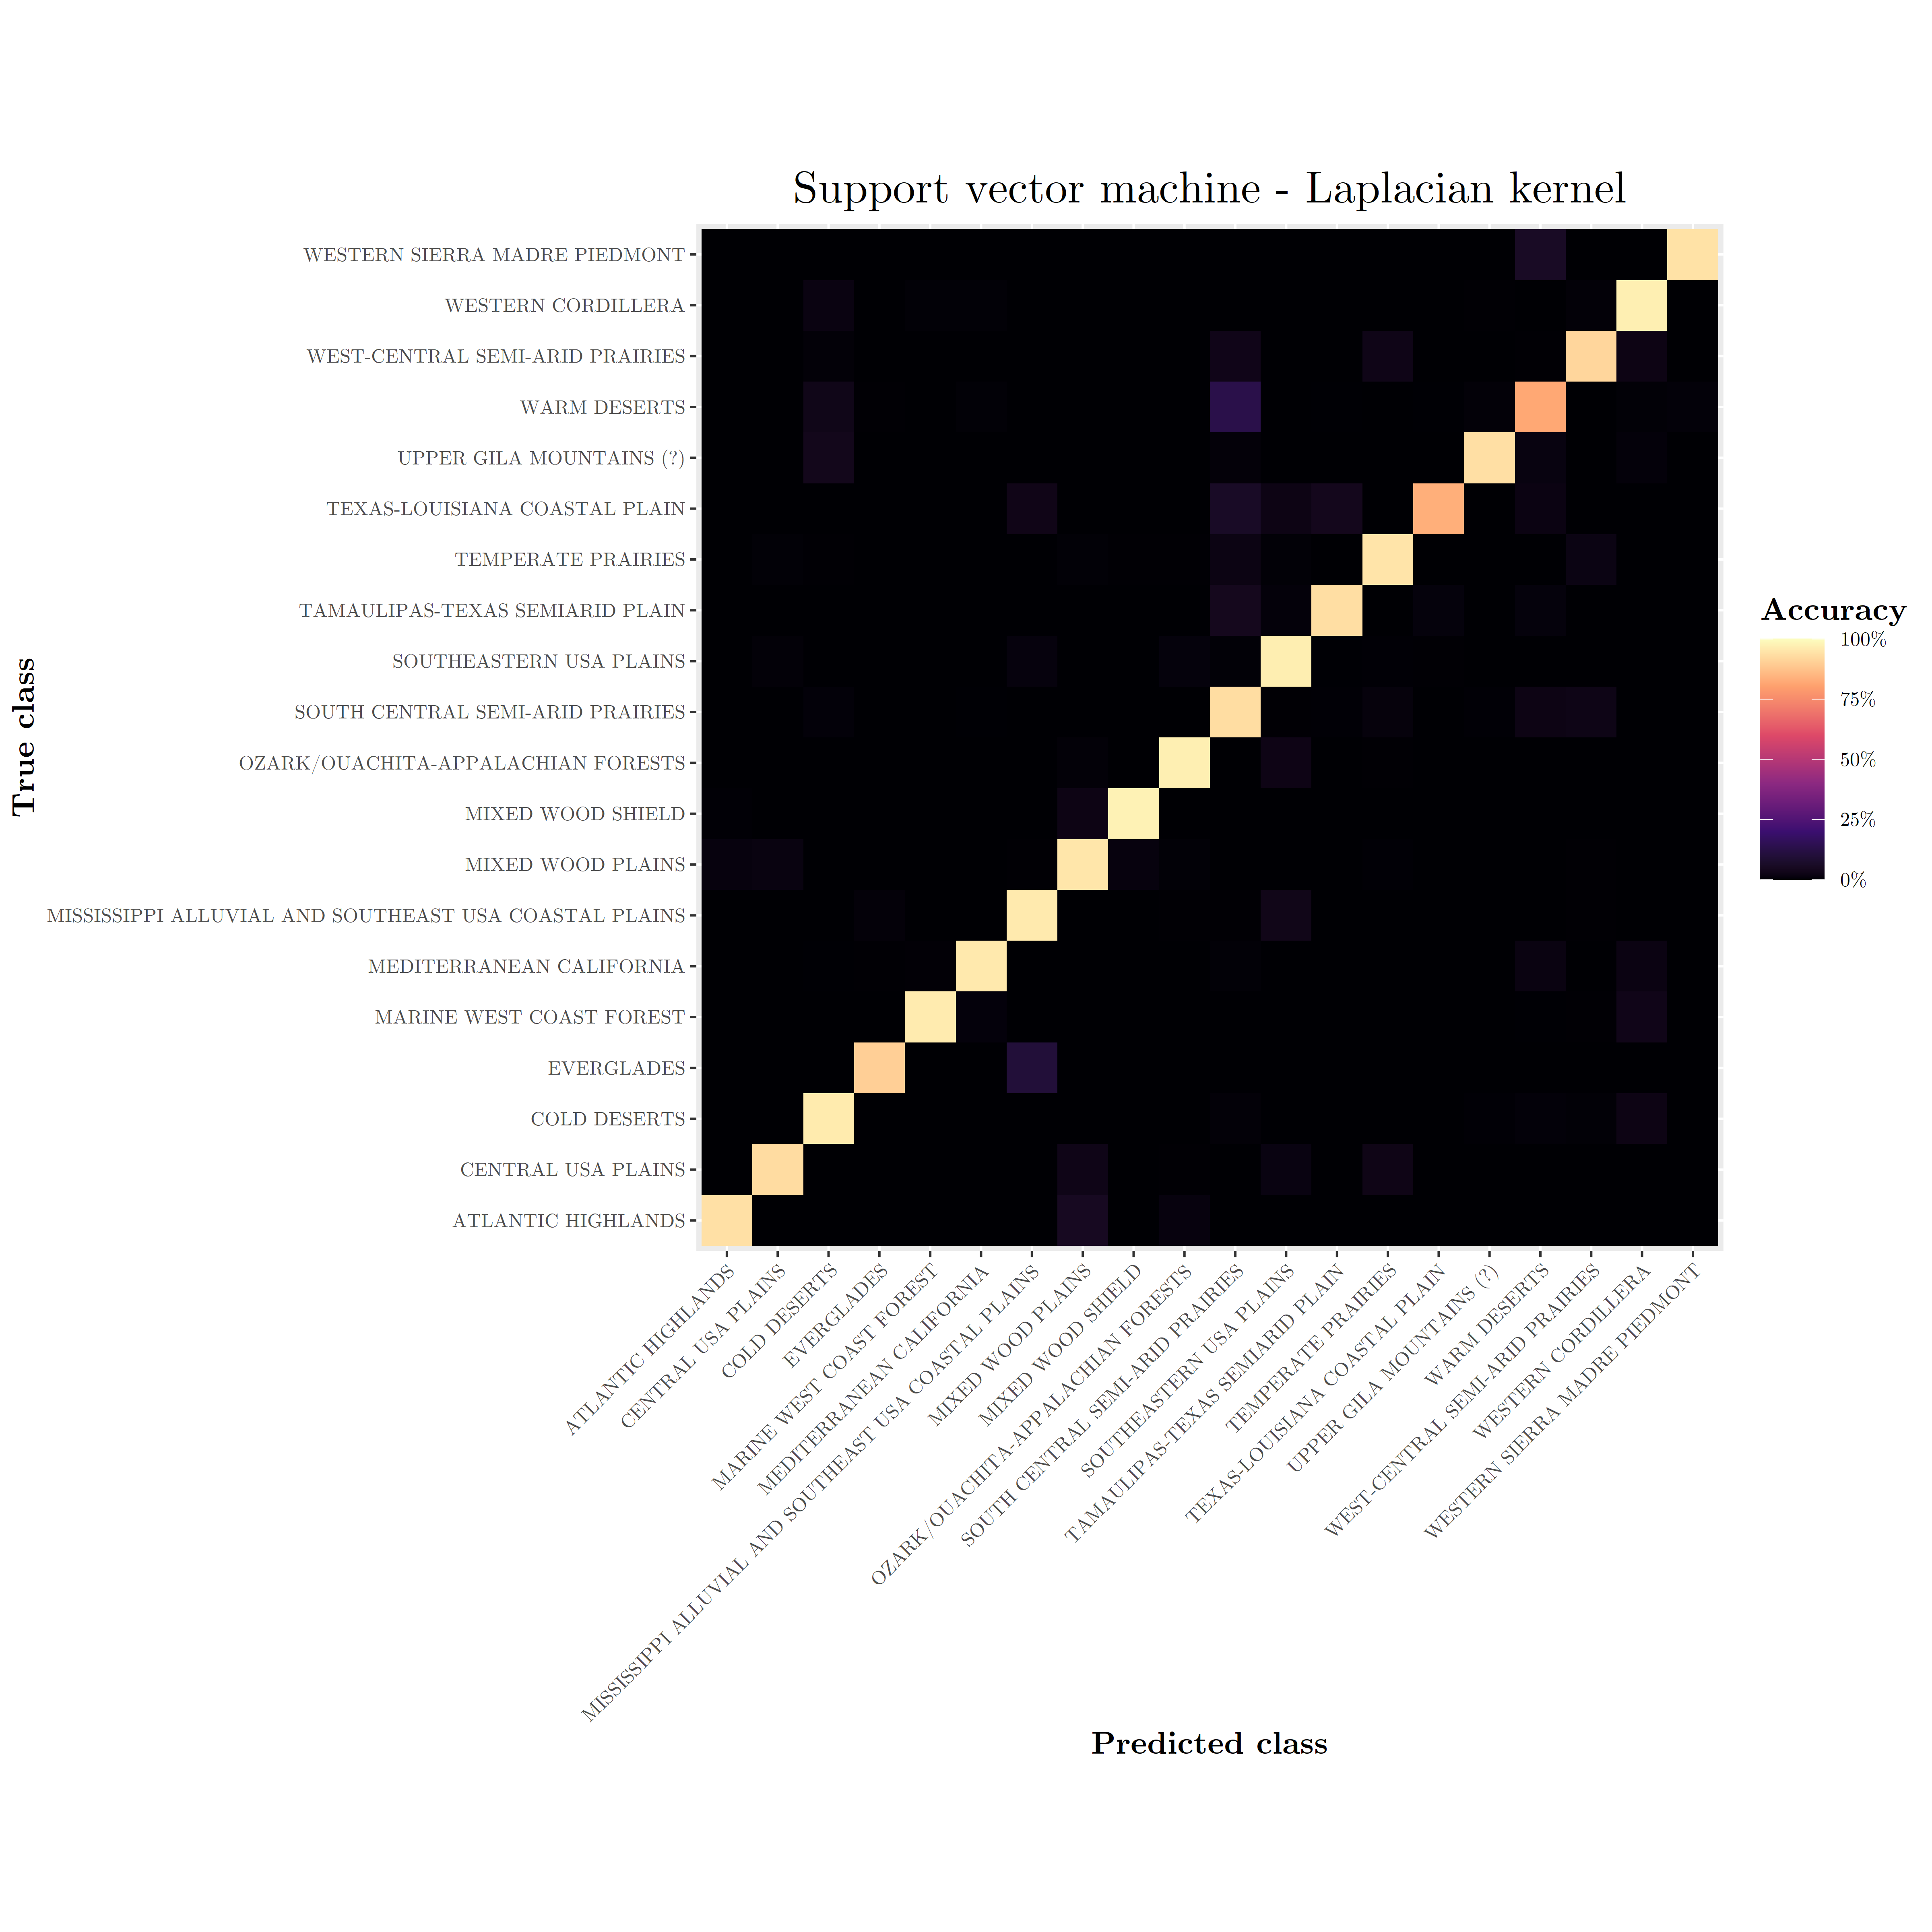
\includegraphics{../Ecosystem discrimination/SVM_confusion_matrix.png}
  \caption{Confusion matrix of the Support Vector Machine model on ecoregion classification. The visualized accuracies are the proportion of the true class being classified as such, the confusion matrix would thus exhibit obvious visible artefacts if the model was overfitting. On the contrary the fact that almost all observations are found on the diagonal shows the voracity of the model and the confirms the validity of using the EPA ecoregions as delineations between distinct assemblages or ecosystems.}
\end{figure}

\newpage

\hypertarget{appendixMaps}{%
\subsection{Raw indices maps}\label{appendixMaps}}

For the figures in the report I have interpolated the values of grid cells with missing functional index values using a inverse distance weighted-mean in a circular sliding window. The original maps are provided here:

\begin{figure}[!h]
  \centering
  \includegraphics[width=\textwidth]{../Final Visualizations/realMap.png}
  \caption{Raw spatial patterns in the topological indices of the functional ecological space. The values for the functional indices (FDis = A\*, FDiv = B\*, FEve = C\*, FRic = D\*) are calculated using the relative weighted mean abundances of species (panel \*1) and presence values (panel \*2).}
  \label{fig:rawMaps}
\end{figure}

\newpage

\hypertarget{appendixSampling}{%
\subsection{East-West Sampling Imbalance}\label{appendixSampling}}

There is significant sampling imbalance in the FIA dataset, as I have visualized here:

\begin{figure}
  \centering
  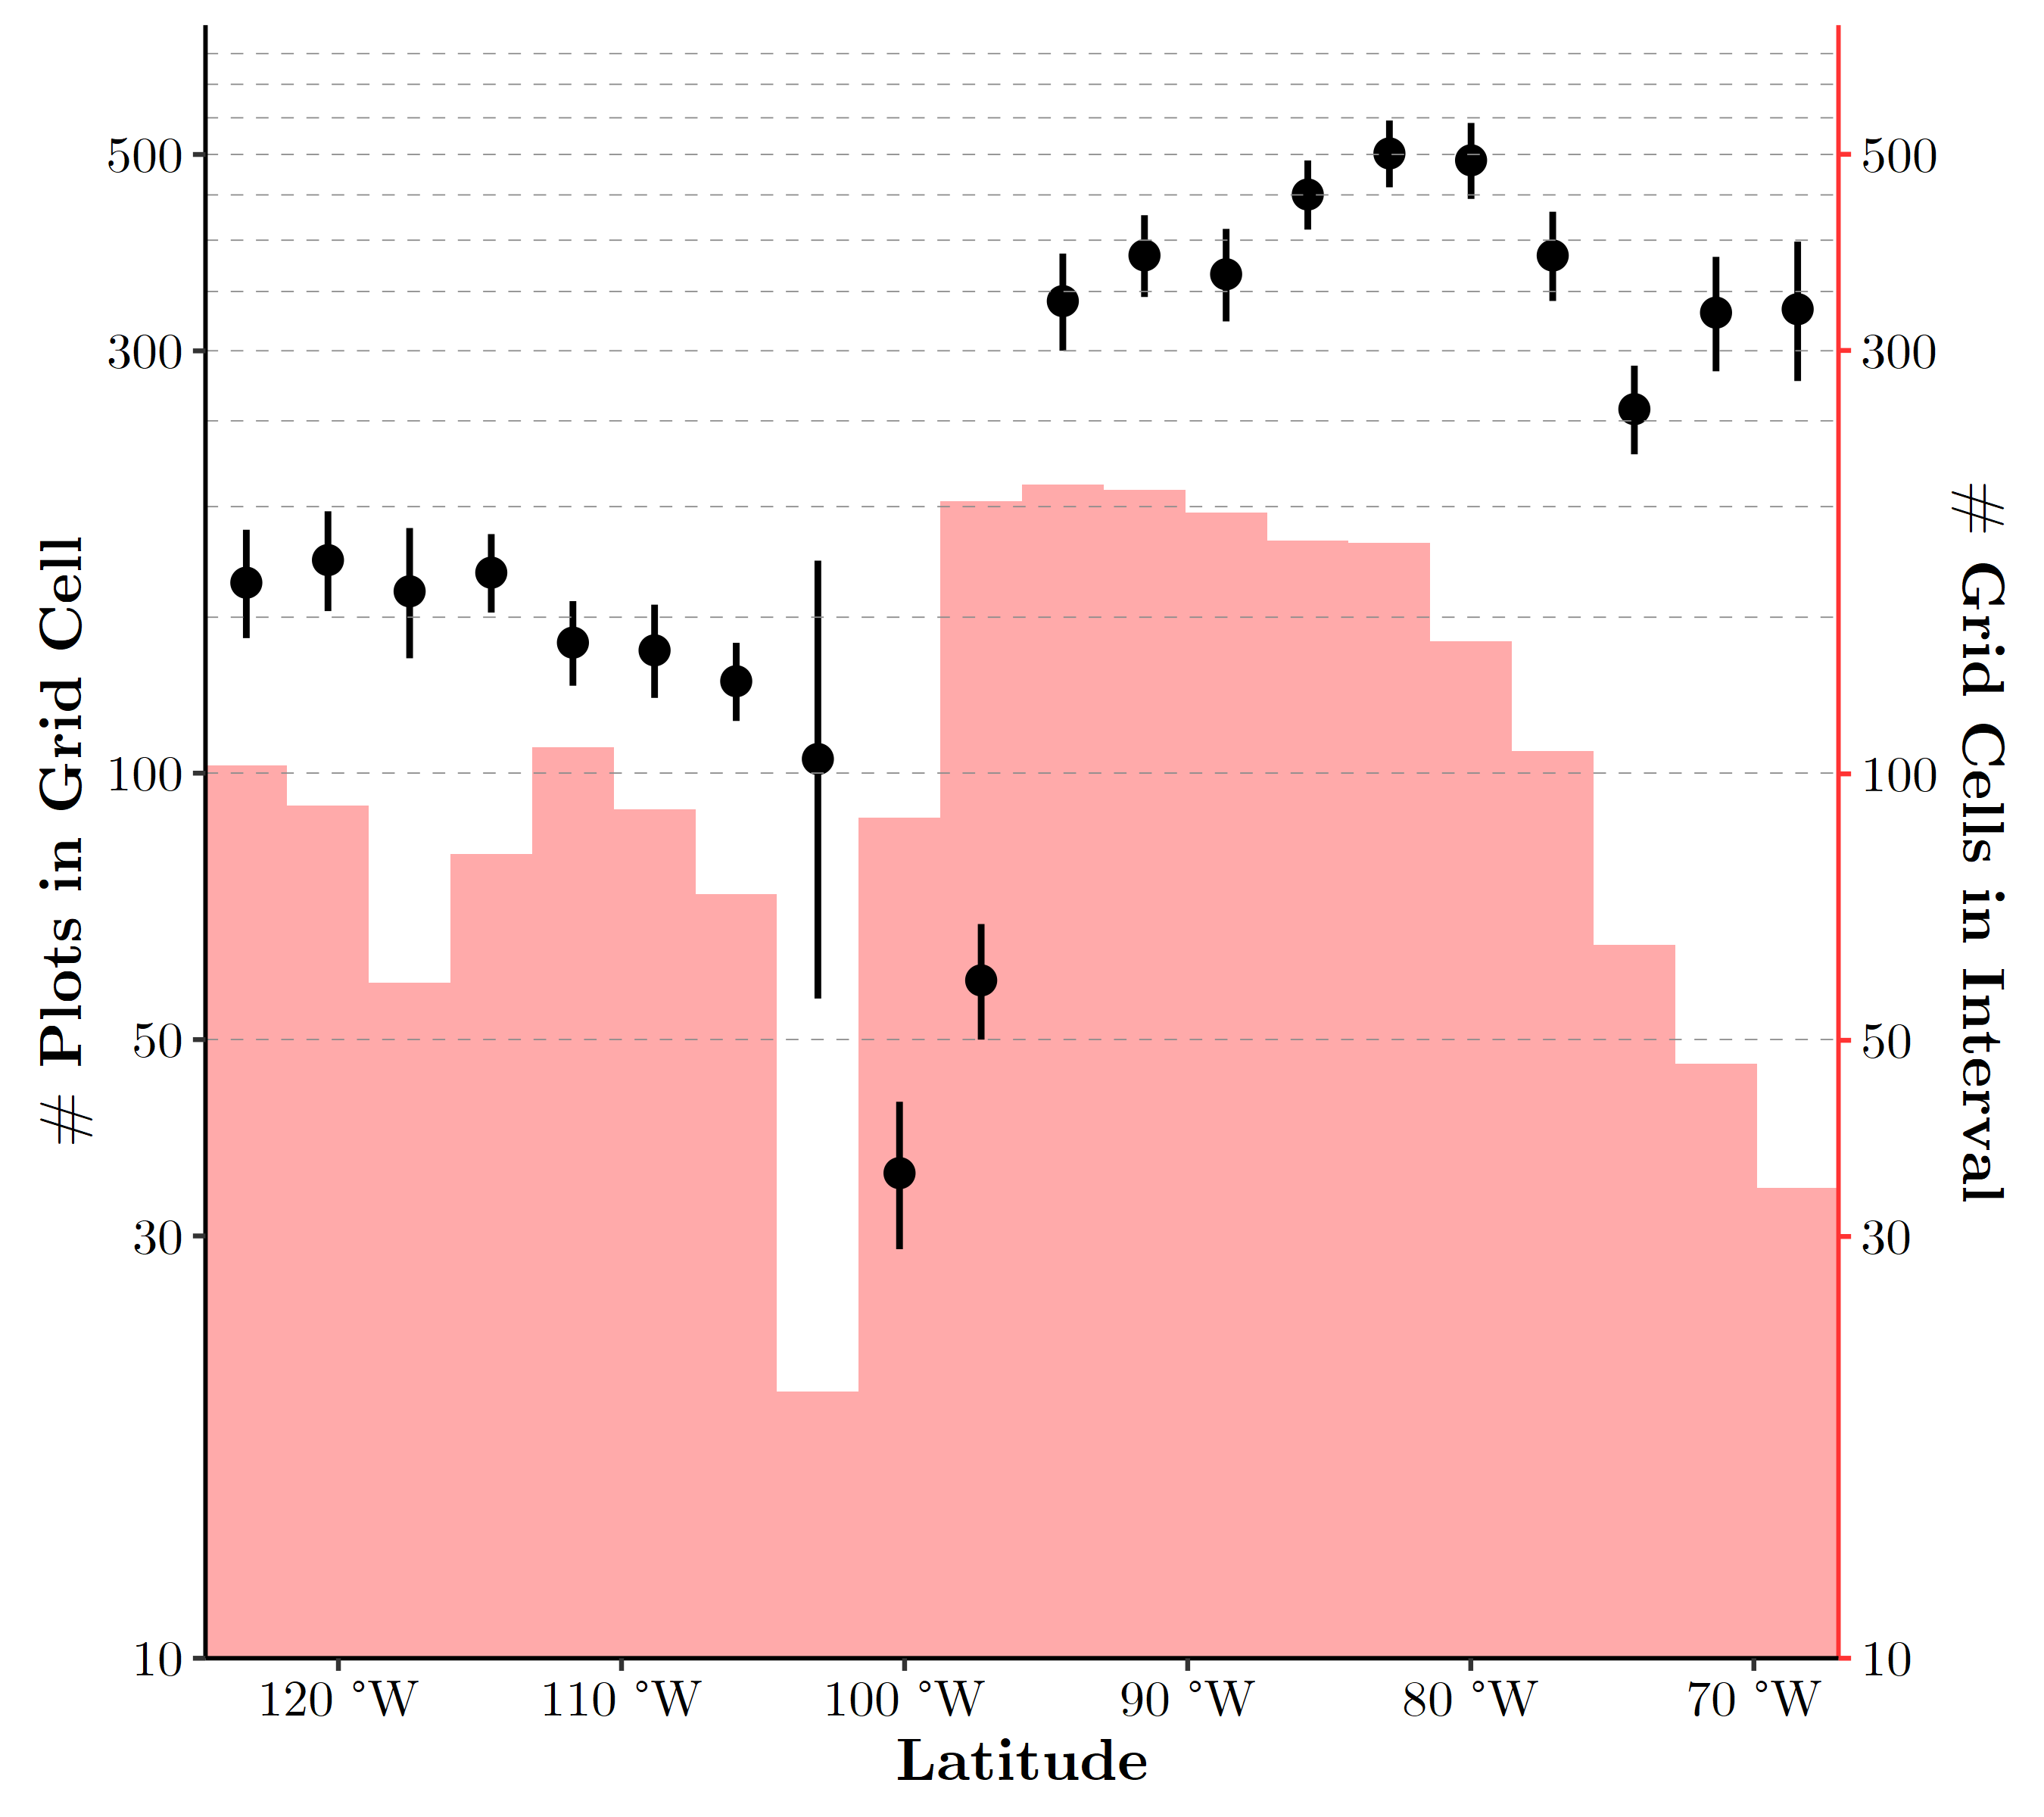
\includegraphics[width=\textwidth]{../Final Visualizations/eastWestSampling.png}
  \caption{East-West sampling imbalance. The black point-ranges are 95\%-confidence intervals of intercept only GLM's on the number of FIA plots per $50 \times 50$km study unit in each latitude interval. The salmon histogram is the number of $50 \times 50$km study unit in each equal interval latitude interval.}
  \label{fig:samplingImbalance}
\end{figure}

\end{document}
